\documentclass{article}

\usepackage{fullpage}
\usepackage{lineno}
\usepackage{wrapfig}
\usepackage{graphicx,color}
\usepackage{amssymb}
\usepackage{subcaption}
\usepackage{braket}
\usepackage{physics}
\usepackage{yquant}
\usepackage{tikz}
\usetikzlibrary{quantikz,fit,quotes,svg.path}
\usepackage[backend=biber,citestyle=numeric-comp]{biblatex}
\ExecuteBibliographyOptions{sorting=nyt,maxbibnames=100,doi=false,isbn=false,url=false}
\addbibresource{cites.bib}

\newcommand{\x}{\textsc{x}}
\newcommand{\cx}{\textsc{cx}}
\newcommand{\ccx}{\textsc{ccx}}
\newcommand{\cccx}{\textsc{cccx}}
\newcommand{\qket}[1]{\ket{\tilde{#1}}}
\newcommand{\preim}[2]{\{\cdot\stackrel{#1}{\longleftarrow}{#2}\}}
\newcommand{\finset}[1]{[\mathbf{#1}]}
\newcommand{\red}[1]{{\color{red}{#1}}}
\newcommand{\todo}[1]{\fbox{\begin{minipage}{40em}{\red{#1}}\end{minipage}}}

\linenumbers

%%%%%%%%%%%%%%%%%%%%%%%%%%%%%%%%%%%%%%%%%%%%%%%%%%%%%%%%%%%%%%%%%%%%%%%%%%%%%%%%%%%%%%%%%%
\title{Classical Symbolic Retrodictive Execution of Quantum Circuits}
\author{Jacques Carette \qquad\qquad Gerardo Ortiz$^{*}$ \qquad\qquad Amr Sabry \\
McMaster University \qquad Indiana University \qquad Indiana University}
\begin{document}
\maketitle

%%%%%%%%%%%%%%%%%%%%%%%%%%%%%%%%%%%%%%%%%%%%%%%%%%%%%%%%%%%%%%%%%%%%%%%%%%%%%%%%%%%%%%%%%%
\begin{refsection}
\section{Main}

%% can double this paragraph in size

\todo{

  small tree width idea suggests we could do retro and measure every
  once in a while. for shor perhaps measure after every iteration of
  multiplication \url{https://arxiv.org/pdf/quant-ph/0511069.pdf}

  try retro with impossible measurement; how happens with the equations:
  retroShor 15 with ancilla=0 produces equation: 0 = 1

  with post selection can we solve SAT ??

  what is know about complexity of converting a circuit to ANF?

  for Shor we construct Uf as part of the algorithm so the cost of
  generating the circuit is part of the complexity analysis

  for the other algos Uf is given to us: if given to us as an ANF
  formula we can answer questions directly with minimal evaluation; so
  the challenge is to convert the Uf box to ANF; exponential in
  general ??? but for the particular functions of interest could be
  efficient

  run Shor backwards from QFT measurement; the state right before QFT
  is a periodic state that approximates the state we would have
  received from forward exec. Good point to discuss existence of
  wavefunction; forward vs backwards. construct circuit with period =
  3; show wavefunction before QFT in regular exec; assume we measure v
  show wavefunction before QFT in retrodictive. Connection between
  these two wavefunctions?

  of course try 1/-1 instead 0/1

  existence of wavefunction: retrodictive QM says no reality to
  wavefunctions.

  other paper on reality of wavefunction; can't be just observer
  belief

  in our work it is an intermediate state of computation, so yes some
  wavefunction exists but which one exists depends on the particulars
  of the execution model and is not uniquely determined by the circuit 

  what would happen in Shor if you put 0 at ancilla init and 1 at
  ancilla measurement (only look for 1 at ancilla measurement)

  post-selection https://en.wikipedia.org/wiki/PostBQP

  why would Nature execute the circuit in the way we draw it

  Use Pi to write circuits because the current model is hardwired to use base 2.

  two classes of variables ???
  Z vars whose values range over 0/1
  X vars whose values range over +/-



We are running classically and symbolically.

State is maintained in ANF.

We will maintain the ANF clauses in p-blocks with a maximum p of say 10.

We will start running with base 2 representation.

  If an operation involves variables in the same block, then good
  
  If an operation involves variables in different blocks, merge the
    blocks, do the operation.
    
  If the block is now too large, find a different basis for this block
    that will make its size smaller
  
---
Step I: QC with qutrits (or more generally qudits)

not x = (x + 1) `mod` 3
cnot (x,y)= (x , (x + y) `mod` 3)
toffoli (x,y,z) = (x , y, (xy + z) `mod` 3)

Bell cnot(x,0) = (x,x)

GHZ  (x,0,0) => (x,x,0) => (x,x,x) 

Shor 21 with qutrits

c0 c1 c2 q0 q1
(0+1+2) (0+1+2) (0+1+2) 0 0
=>
(c2,q1) c0 c1 q0
(00+11+22) (0+1+2) (0+1+2) 0 
=>
(c1,c2,q1) c0 q0
(000+112+221) (0+1+2) 0
=>
(c1,c2,q1,q0) c0 
(0000+1122+2211) (0+1+2)
=>
(c1,c2,q1,q0) c0 
(0000+1112+2201) (0+1+2)
=>
(c1,c2,q1,q0) c0 
(0000+1110+2201) (0+1+2)
=>
(c1,c2,q1,q0) c0 
(0010+1120+2211) (0+1+2)
=>
(c0,c1,c2,q1,q0) 
(00010+01120+02211+10011+11122+12212+20012+21121+22210)
=>
(c0,c1,c2,q1,q0) 
(00020+01100+02221+10021+11102+12222+20022+21101+22220)
=>
(c0,c1,c2,q1,q0) 
(00022+01100+02220+10020+11102+12221+20021+21101+22222)
=>
(c0,c1,c2,q1,q0) 
(00022+01100+02220+10020+11122+12201+20011+21121+22202)
=>
(c0,c1,c2,q1,q0) 
(00021+01100+02222+10022+11121+12201+20012+21120+22202)


c0 c1 c2 q0 q1	

01100 +

21102 +

12210 +

00012 +
11112 +

22220

20021 +

02222 +
10022 +





---

Need to write quantum programs in a way that is independent of the
underlying basis and let the runtime system change basis to reduce the
size of the intermediate states.

This could be related to QFT and to reducing dimension in ML

Circuit for 4^x mod 21

x    f(x)
0    1
1    4
2    16
3    1
4    4
5    16
6    1
7    4

3 qubits for computational register (c2c1c0)
5 qubits for ancilla (a4a3a2a1a0)

000 00000  ==> 000 00001
001 00000  ==> 001 00100
010 00000  ==> 010 10000
011 00000  ==> 011 00001
100 00000  ==> 100 00100
101 00000  ==> 101 10000
110 00000  ==> 110 00001
111 00000  ==> 111 00100

000 + 011 + 110 ==> a0=1
001 + 100 + 111 ==> a2=1
010 + 101       ==> a4=1

cccx(-c2,-c1,-c0,a0)
cccx(-c2,c1,c0,a0)
cccx(c2,c1,-c0,a0)
cccx(-c2,-c1,c0,a2)
cccx(c2,-c1,-c0,a2)
cccx(c2,c1,c0,a2)
cccx(-c2,c1,-c0,a4)
cccx(c2,-c1,c0,a4)

--- Execute keeping track of blocks (keep max at 4)

{c2} {c1} {c0} {a4} {a3} {a2} {a1} {a0}
     (0+1)(0+1)(0+1) 00000

{c2,c1,c0,a0} {a4} {a3} {a2} {a1}
 (0001+0010+0100+0110+1000+1010+1100+1110) 0000
 (0001+0010+0100+0111+1000+1010+1100+1110) 0000
 (0001+0010+0100+0111+1000+1010+1101+1110) 0000

{c2,c1,c0,a0,a2} {a4} {a3} {a1}
 (00010+00101+01000+01110+10000+10100+11010+11100) 000
 express 2+5+8+14+16+20+26+28 in base 3
 00002+00012+00022+00112+00121+00202+00222+01001
 0 (0002+0012+0022+0112+0121+0202+0222+1001)

{c2} {c1,c0,a0,a2} {a4} {a3} {a1}






--- Symbolically ?


}

start with base 2 (booleans) and maximum groups of p.
if groups get too big switch to another basis that makes the representation smaller
related to p-adics ???


Retrodictive quantum theory~\cite{sym13040586},
retrocausality~\cite{Aharonov2008}, and the time-symmetry of physical
laws~\cite{RevModPhys.27.179} suggest that partial knowledge about the
future can be exploited to understand the present. We demonstrate the
even stronger proposition that, in concert with the computational
concepts of \emph{demand-driven lazy evaluation}~\cite{lazyevaluator}
and \emph{symbolic partial evaluation}~\cite{futamura}, retrodictive
reasoning can be used as a computational resource to de-quantize some
quantum algorithms, i.e., to provide efficient classical algorithms
inspired by their quantum counterparts.

\paragraph*{Symbolic Execution of Classical Programs Applied to Quantum Oracles.}
A well-established technique to simultaneously explore multiple paths
that a classical program could take under different inputs is
\emph{symbolic
  execution}~\cite{10.1145/390016.808445,10.1145/360248.360252,howden,10.1145/800191.805647,10.1145/3182657}. In
this execution scheme, concrete values are replaced by symbols which are
initially unconstrained. As the execution proceeds, the symbols
interact with program constructs and this typically introduces
constraints on the possible values that the symbols represent. At the
end of the execution, these constraints can be solved to infer
properties of the program under consideration. The idea is also
applicable to quantum circuits as the following example illustrates.

\begin{wrapfigure}{r}{9cm}
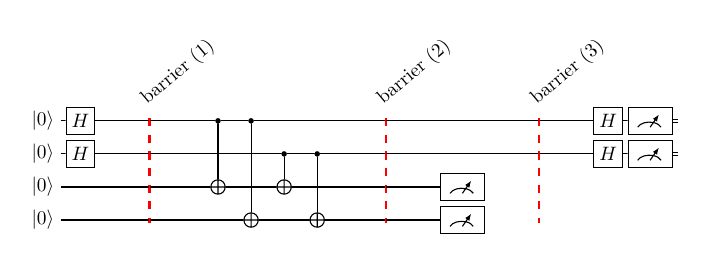
\begin{tikzpicture}[scale=0.7,every label/.style={rotate=40, anchor=south west}]
\begin{yquant*}[operators/every barrier/.append style={red, thick}]

    qubit {$\ket0$} a0;
    qubit {$\ket0$} a1;
    qubit {$\ket0$} b0;
    qubit {$\ket0$} b1;
    
    box {$H$} a0;
    box {$H$} a1;
    
    ["barrier (1)"]
    barrier (-);

    cnot b0 | a0;
    cnot b1 | a0;
    cnot b0 | a1;
    cnot b1 | a1;

    ["barrier (2)"]
    barrier (-);

    measure b0;
    measure b1;
    discard b0;
    discard b1;

    ["barrier (3)"]
    barrier (-);

    box {$H$} a0;
    box {$H$} a1;
    measure a0;
    measure a1;
\end{yquant*}
\end{tikzpicture}
\caption{\label{fig:Simon}Circuit for Simon's Algorithm $n=2$ and $a=3$}
\end{wrapfigure}
Let $\finset{n}$ denote the finite set $\{ 0,1,\ldots,(n-1)\}$. In
Simon's problem, we are given a 2-1 (classical) function $f :
\finset{2^n} \rightarrow \finset{2^n}$ with the property that there
exists an $a$ such $f(x) = f(x \oplus a)$ for all~$x$; the goal is to
determine~$a$. The circuit in Fig.~\ref{fig:Simon} implements the
quantum algorithm when $n=2$ and $a = 3$. In the circuit, the gates
between barriers (1) and (2) implement a quantum oracle $U_f(x,0) =
(x,f(x))$ that encapsulates the function $f$ of interest. A direct
classical simulation of the quantum circuit would need to execute the
$U_f$ block four times, once for each possible value $\ket{00}$,
$\ket{01}$, $\ket{10}$, and~$\ket{11}$ for the top two wires. Instead,
let us introduce two symbols $x_0$ representing the top wire and~$x_1$
representing the wire below it, and let's proceed with the execution
symbolically. The state at barrier (1) is initially
$\ket{x_0x_100}$. At the first \cx-gate, we symbolically calculate the
result of the target wire as $x_0 \oplus 0 = x_0$ evolving the state
to $\ket{x_0x_1x_00}$. Going through the next three \cx-gates, the
state evolves as $\ket{x_0x_1x_0x_0}$, $\ket{x_0x_1(x_0\oplus
  x_1)x_0}$, and $\ket{x_0x_1(x_0\oplus x_1)(x_0\oplus x_1)}$ at
barrier~(2). At that point, we have established that the bottom two
wires are equal; the result of their measurement can only be $00$ or
$11$. Since the function is promised to be 2-1 for all inputs, it is
sufficient to analyze one case, say when the measurement at barrier
(3) produces $00$. This measurement collapses the top wires to
$\ket{x_0x_1}$ subject to the constraint that $x_0\oplus x_1 = 0$ or
equivalently that $x_0 = x_1$.  We have thus inferred that both
$x_0=x_1=0$ and $x_0=x_1=1$ produce the same measurement result at
barrier (3) and hence that $f(00) = f(11) = f(00 \oplus 11)$ which
reveals that $a$ is~$11$ in binary notation.

Since the quantum circuit between barriers (1) and (2) is reversible,
we can perform the analysis above in a mixed predictive and symbolic
retrodictive execution to make the flow of information conceptually
clearer. We start a forward classical simulation with one arbitrary
state at barrier (1), say $\ket{0100}$.  This state evolves to
$\ket{0100}$, then $\ket{0100}$ again, then $\ket{0110}$, and finally
$\ket{0111}$. In this case, the result of measuring the bottom two
wires is $11$. Having produced a possible measurement at barrier (3),
we start a retrodictive execution to find out what other input states
might be compatible with this future measurement. To that end, we
execute the circuit backwards with the symbolic state
$\ket{x_0x_111}$; that execution evolves to $\ket{x_0x_11(1\oplus
  x_1)}$, then $\ket{x_0x_1(1\oplus x_1)(1\oplus x_1)}$, then
$\ket{x_0x_1(1\oplus x_1)(1\oplus x_0 \oplus x_1)}$, and finally
$\ket{x_0x_1(1\oplus x_0 \oplus x_1)(1\oplus x_0 \oplus x_1)}$. Having
reached the initial conditions on the bottom two wires, we reconcile
them with the collected constraints to conclude that $1 \oplus x_0
\oplus x_1 = 0$ or equivalently that $x_0 \neq x_1$. The measurement
of 11 at barrier~(3) is consistent with not just the state $\ket{01}$
we started with but also with the state $\ket{10}$. In other words, we
have $f(01) = f(10) = f(01 \oplus 11)$ and the hidden value of $a$ is
revealed to be $11$.

\begin{figure}[t]
  \begin{subfigure}{0.5\textwidth}
  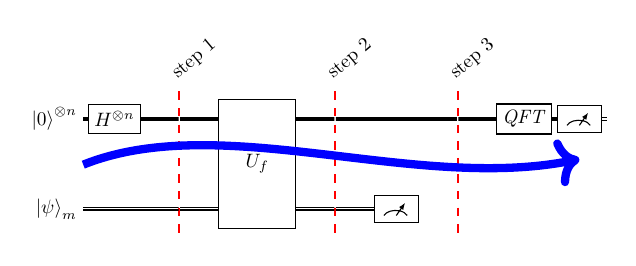
\begin{tikzpicture}[scale=0.7,every label/.style={rotate=40, anchor=south west}]
    \begin{yquant*}[operators/every barrier/.append style={red, thick},
        operator/minimum width=7mm,
        operator/separation=1mm,
        register/separation=10mm]
    qubits {$\ket0^{\otimes n}$} a;
    qubits {$\ket{\psi}_m$} b;
    box {$H^{\otimes n}$} a;
    ["step 1"]
    barrier (-);
    [x radius=7mm, y radius=7mm]
    box {$U_f$} (a,b);
    ["step 2"]
    barrier (-);
    measure b;
    discard b;
    ["step 3"]
    barrier (-);
    box {$\mathit{QFT}$} a;
    measure a;
    \end{yquant*}
    \draw[line width=3pt, ->, blue] (0,-1.1) .. controls (2.5,-0.1) and (6,-1.6) .. (9,-1);
  \end{tikzpicture}
  \caption{Conventional Flow}
  \end{subfigure}
  \begin{subfigure}{0.5\textwidth}
  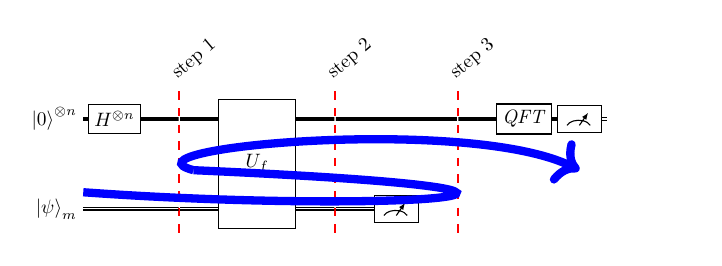
\begin{tikzpicture}[scale=0.7,every label/.style={rotate=40, anchor=south west}]
    \begin{yquant*}[operators/every barrier/.append style={red, thick},
        operator/minimum width=7mm,
        operator/separation=1mm,
        register/separation=10mm]
    qubits {$\ket0^{\otimes n}$} a;
    qubits {$\ket{\psi}_m$} b;
    box {$H^{\otimes n}$} a;
    ["step 1"]
    barrier (-);
    [x radius=7mm, y radius=7mm]
    box {$U_f$} (a,b);
    ["step 2"]
    barrier (-);
    measure b;
    discard b;
    ["step 3"]
    barrier (-);
    box {$\mathit{QFT}$} a;
    measure a;
  \end{yquant*}
  \draw[line width=3pt, blue] (0,-1.6) .. controls (5.5,-2) and (11,-1.6) .. (2,-1.2);
  \draw[line width=3pt, ->, blue] (2,-1.2) .. controls (0.5,-0.8) and (7,-0.2) .. (9,-1.2);
  \end{tikzpicture}
  \caption{Retrodictive Flow}
  \end{subfigure}
\caption{\label{fig:templateQC}Template quantum circuit}
\end{figure}
\begin{wrapfigure}{r}{3cm}
\begin{center}
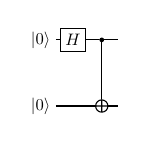
\begin{tikzpicture}[scale=0.6]
   \begin{yquant*}[register/minimum height=1.3cm]
   qubit {$\ket0$} x;
   qubit {$\ket0$} y;
   box {$H$} x;
   cnot y | x;
  \end{yquant*}
\end{tikzpicture}
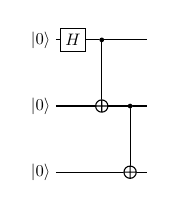
\begin{tikzpicture}[scale=0.6]
   \begin{yquant*}[register/minimum height=1.3cm]
   qubit {$\ket0$} x;
   qubit {$\ket0$} y;
   qubit {$\ket0$} z;
   box {$H$} x;
   cnot y | x;
   cnot z | y;
  \end{yquant*}
\end{tikzpicture}
\end{center}
\caption{\label{fig:bell}Bell and GHZ States}
\end{wrapfigure}
\paragraph*{Representing Wavefunctions Symbolically.}
A symbolic variable represents a boolean value that can be 0 or 1;
this is similar to a qubit in a superposition $(1/\sqrt{2}) (\ket{0}
\pm \ket{1})$. Thus, it appears that $H\ket{0}$ could be represented
by a symbol~$x$ to denote the uncertainty. Surprisingly, this idea
scales to even represent maximally entangled
states. Fig.~\ref{fig:bell}(left) shows a circuit to generate the Bell
state $(1/\sqrt{2}) (\ket{00} + \ket{11})$. By using the symbol $x$
for $H\ket{0}$, the input to the \cx-gate is $\ket{x0}$ which
evolves to $\ket{xx}$. By sharing the same symbol in two positions,
the symbolic state accurately represents the entangled Bell
state. Similarly, for the circuit in Fig.~\ref{fig:bell}(right), the
state after the Hadamard gate is $\ket{x00}$ which evolves to
$\ket{xx0}$ and then to $\ket{xxx}$ again accurately capturing the
entanglement correlations.

\todo{ need for entanglement~\cite{10.2307/3560059}
  }



This insight allows us to symbolically execute the many quantum
algorithms that match the template in Fig.~\ref{fig:templateQC}
(including Deutsch, Deutsch-Jozsa, Bernstein-Vazirani, Simon, Grover,
and Shor's algorithms). Specifically, in all these algorithms, the top
collection of wires (which we will call the computational register) is
prepared in a uniform superposition which can be represented using
symbolic variables. Below, we report on the results of such symbolic
executions. In each case, instead of the conventional execution flow
depicted in Fig.~\ref{fig:templateQC}(a), we find a possible
measurement outcome $w$ at barrier (3) and perform a retrodictive
execution with a state $\ket{xw}$ going backwards to collect the
constraints on $x$ that enable us to solve the problem in question.

\begin{wrapfigure}{r}{4cm}
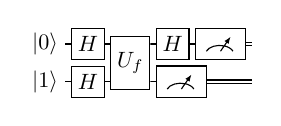
\begin{tikzpicture}[scale=0.8]
   \begin{yquant*}
   qubit {$\ket0$} x;
   qubit {$\ket1$} y;
   box {$H$} x;
   box {$H$} y;
   box {$U_f$} (x,y);
   measure y;
   box {$H$} x;
   measure x;
  \end{yquant*}
\end{tikzpicture}
\caption{\label{fig:deutsch}Deutsch}
\end{wrapfigure}
\paragraph*{Deutsch.} The quantum circuit in Fig.~\ref{fig:deutsch} determines
if the function $\finset{2} \rightarrow \finset{2}$ encapsulated in
the quantum oracle $U_f$ is constant or balanced. Since 0 is always a
possible measurement of the ancilla register, we start a retrodictive
execution of the $U_f$ block with state $\ket{x0}$. This execution
terminates with a state $\ket{xr}$ where $r$ is a formula expressing
the dependencies of the ancilla on~$x$. Running the experiment with
different choices for $f$, the resulting formula always perfectly
describes $f$. Specifically when $f$ is the constant function that
returns 0, we have $r=0$; when $f$ is the constant function that
returns 1, we have $r=0$; when $f$ is the balanced function that
returns its input, we have $r=x$; and when $f$ is the balanced function that
returns the negation of its input, we have $r=1\oplus x$.

\paragraph*{Deutsch-Jozsa.} 
The problem is a generalization of the previous one. We are given a
function $\finset{2^n} \rightarrow \finset{2}$ that is promised to be
constant or balanced and we need to decide distinguish the two
cases. The quantum circuit generalizes the one in
Fig.~\ref{fig:deutsch} to use $n$-wires for the computation
register. Similarly to before, we perform a retrodictive execution of
the $U_f$ block with the state $\ket{x_{n-1}\cdots x_1x_00}$ and
observe the resulting formula $r$. Like before, when the function is
constant, the formula $r$ is the corresponding constant and when the
function is balanced, the formula $r$ completely describes how the
result is computed from the symbols $x_{n-1},\cdots,x_1,x_0$. For
example, for $n=6$, the resulting formulae for three balanced
functions were: $x_0$, $x_0 \oplus x_1 \oplus x_2 \oplus x_3 \oplus
x_4 \oplus x_5$, and $1 \oplus x_3x_5 \oplus x_2x_4 \oplus x_1x_5
\oplus x_0x_3 \oplus x_0x_2 \oplus x_3x_4x_5 \oplus x_2x_3x_5 \oplus
x_1x_3x_5 \oplus x_0x_3x_5 \oplus x_0x_1x_4 \oplus x_0x_1x_2 \oplus
x_2x_3x_4x_5 \oplus x_1x_3x_4x_5 \oplus x_1x_2x_4x_5 \oplus
x_1x_2x_3x_5 \oplus x_0x_3x_4x_5 \oplus x_0x_2x_4x_5 \oplus
x_0x_2x_3x_5 \oplus x_0x_1x_4x_5 \oplus x_0x_1x_3x_5 \oplus
x_0x_1x_3x_4 \oplus x_0x_1x_2x_4 \oplus x_0x_1x_2x_4x_5 \oplus
x_0x_1x_2x_3x_5 \oplus x_0x_1x_2x_3x_4$. In the first case, the
function is balanced because its output depends on just one variable
(which is 0 in half the possible inputs); in the second case the
output of the function is the exclusive-or of all the input variables
which is an easy instance of a balanced function. The last case is a
cryptographically strong balanced function whose output pattern is, by
design, difficult to discern~\cite{quteprints21763}. An important
insight in the case of the Deutsch-Jozsa problem is that, since we are
promised the function is either constant or balanced, then any formula
that refers to at least one variable must indicate a balanced
function. In other words, the outcome of the algorithm can be
immediately decided if the formula is anything other than 0 or 1. We
confirmed this observation by running the experiment on all 12870
balanced functions from $\finset{2^4} \rightarrow \finset{2}$ and
correctly identifying them as such. This is significant as some of
these functions produce complicated entangled patterns during quantum
evolution and could not be de-quantized using previous
approaches~\cite{djdeq}. The catch is that symbolic retrodictive
execution is not consistent with ``query complexity'' as it operates
in time proportional to the depth of the quantum oracle and the size
of the formula.


\begin{wrapfigure}{r}{7cm}
  \begin{center}
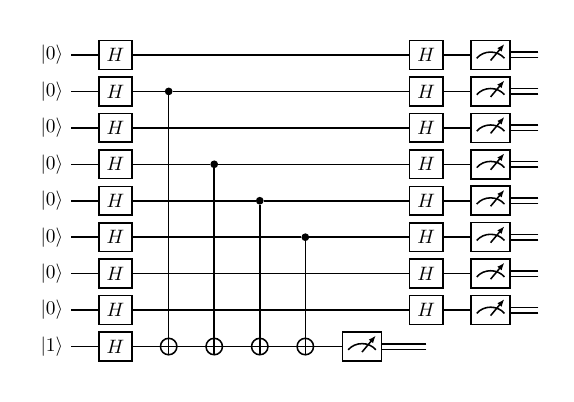
\begin{tikzpicture}\node[scale=0.7]{
\begin{quantikz}[row sep=0.02cm]\label{eq:bernstein-vazirani}
   \lstick{$\ket{0}$} & \gate{H} & \qw      & \qw      & \qw       & \qw       & \qw & \gate{H} 
   & \meter{} & \cw \\
   \lstick{$\ket{0}$} & \gate{H} & \ctrl{7} & \qw      & \qw       & \qw       & \qw & \gate{H} 
   & \meter{} & \cw \\
   \lstick{$\ket{0}$} & \gate{H} & \qw      & \qw      & \qw       & \qw       & \qw & \gate{H} 
   & \meter{} & \cw \\
   \lstick{$\ket{0}$} & \gate{H} & \qw      & \ctrl{5} & \qw       & \qw       & \qw & \gate{H} 
   & \meter{} & \cw \\
   \lstick{$\ket{0}$} & \gate{H} & \qw      & \qw      & \ctrl{4}  & \qw       & \qw & \gate{H} 
   & \meter{} & \cw \\
   \lstick{$\ket{0}$} & \gate{H} & \qw      & \qw      & \qw       & \ctrl{3}  & \qw & \gate{H} 
   & \meter{} & \cw \\
   \lstick{$\ket{0}$} & \gate{H} & \qw      & \qw      & \qw       & \qw       & \qw & \gate{H} 
   & \meter{} & \cw \\
   \lstick{$\ket{0}$} & \gate{H} & \qw      & \qw      & \qw       & \qw       & \qw & \gate{H} 
   & \meter{} & \cw \\
   \lstick{$\ket{1}$}  & \gate{H}  & \targ{}  & \targ{}  & \targ{}   & \targ{}   & \meter{} 
   & \cw
\end{quantikz}
};\end{tikzpicture}
\end{center}
\caption{\label{fig:bv}Circuit for Bernstein-Vazirani
  Algorithm ($n=8$, $s=92$, least significant bit is the top wire)}
\end{wrapfigure}
\paragraph*{Bernstein-Vazirani.} 
We are given a function $f : \finset{2^n} \rightarrow \finset{2}$ that
hides a secret number $s \in \finset{2^n}$. We are promised the
function is defined using the binary representations $\sum_i^{n-1}
x_i$ and $\sum_i^{n-1} s_i$ of $x$ and $s$ respectively as $f(x) =
\sum_{i=0}^{n-1} s_ix_i \mod{2}$.  The goal is to determine the secret
number $s$. The circuit in Fig.~\ref{fig:bv} solves the problem for
$n=8$ and a hidden number 92 ($= 00111010$ in binary notation with the
rightmost bit at index 0). Retrodictive execution starting with the
state $\ket{x_0x_1x_2x_3x_4x_5x_6x_70}$ terminates with the formula
$x_1 \oplus x_3 \oplus x_4 \oplus x_5$. The secret string can be
immediately read from the formula as the indices $\{ 1,3,4,5 \}$ of
the symbols are exactly the positions at which the secret string has a
1.

\begin{figure}
\begin{tabular}{ll}
$u=0$ & 
  $1 \oplus x_3 \oplus x_2 \oplus x_1 \oplus x_0 \oplus x_2x_3 \oplus x_1x_3 \oplus x_1x_2 \oplus x_0x_3 \oplus x_0x_2 \oplus x_0x_1 \oplus x_1x_2x_3 \oplus x_0x_2x_3$ \\
   &\quad $\oplus ~x_0x_1x_3 \oplus x_0x_1x_2 \oplus x_0x_1x_2x_3$ \\
$u=1$ & 
  $x_0 \oplus x_0x_3 \oplus x_0x_2 \oplus x_0x_1 \oplus x_0x_2x_3 \oplus x_0x_1x_3 \oplus x_0x_1x_2 \oplus x_0x_1x_2x_3$ \\
$u=2$ &
  $x_1 \oplus x_1x_3 \oplus x_1x_2 \oplus x_0x_1 \oplus x_1x_2x_3 \oplus x_0x_1x_3 \oplus x_0x_1x_2 \oplus x_0x_1x_2x_3$ \\
$u=3$ &
  $x_0x_1 \oplus x_0x_1x_3 \oplus x_0x_1x_2 \oplus x_0x_1x_2x_3$ \\
$u=4$ &
  $x_2 \oplus x_2x_3 \oplus x_1x_2 \oplus x_0x_2 \oplus x_1x_2x_3 \oplus x_0x_2x_3 \oplus x_0x_1x_2 \oplus x_0x_1x_2x_3$ \\
$u=5$ &
  $x_0x_2 \oplus x_0x_2x_3 \oplus x_0x_1x_2 \oplus x_0x_1x_2x_3$ \\
$u=6$ &
  $x_1x_2 \oplus x_1x_2x_3 \oplus x_0x_1x_2 \oplus x_0x_1x_2x_3$ \\
$u=7$ &
  $x_0x_1x_2 \oplus x_0x_1x_2x_3$ \\
$u=8$ &
  $x_3 \oplus x_2x_3 \oplus x_1x_3 \oplus x_0x_3 \oplus x_1x_2x_3 \oplus x_0x_2x_3 \oplus x_0x_1x_3 \oplus x_0x_1x_2x_3$ \\
$u=9$ &
  $x_0x_3 \oplus x_0x_2x_3 \oplus x_0x_1x_3 \oplus x_0x_1x_2x_3$ \\
$u=10$ &
  $x_1x_3 \oplus x_1x_2x_3 \oplus x_0x_1x_3 \oplus x_0x_1x_2x_3$ \\
$u=11$ &
  $x_0x_1x_3 \oplus x_0x_1x_2x_3$ \\
$u=12$ &
  $x_2x_3 \oplus x_1x_2x_3 \oplus x_0x_2x_3 \oplus x_0x_1x_2x_3$ \\
$u=13$ &
  $x_0x_2x_3 \oplus x_0x_1x_2x_3$ \\
$u=14$ &
  $x_1x_2x_3 \oplus x_0x_1x_2x_3$ \\
$u=15$ &
  $x_0x_1x_2x_3$
\end{tabular}
\caption{\label{fig:Grover}Result of retrodictive execution for the Grover oracle ($n=4$, $w$ in the range $\{0..15\}$).}
\end{figure}


\paragraph*{Grover.}  We are given a function $f : \finset{2^n}
\rightarrow \finset{2}$ with the property that there exists only one
input $u$ such $f(u) = 1$. The goal is to find $u$. The conventional
presentation of the quantum algorithm does not fit the template of
Fig.~\ref{fig:templateQC}. But it is still possible to construct a
quantum oracle $U_f$ from the given $f$ and perform retrodictive
execution starting from an ancilla measurement of 1 corresponding to
the input pattern we are interested in. The resulting equations for
$n=4$ and $u$ in the range $\{0..15\}$ are in
Fig.~\ref{fig:Grover}. In some cases (e.g. $u=15$) the equations
immediately reveal $u$; in others, retrodictive executive provides no
advantage since solving arbitrary equations over boolean variables is,
in general, an $\mathit{NP}$-complete problem.

\todo{
  run PEZ with +1/-1 instead of 0/1


  black box model forbids you to use some interesting property of the
  circuit for $U_f$; we actually have this too because ANF
  representation does not depend on how you implement the
  circuit. (circuit for $a^x \mod{15}$ manually optimized or not gives
  the same formula); so we could fit in the black box model but
  putting the formula inside the black box. We can answer lots of
  questions quickly but not Shor in general.

  if oracle takes n steps to answer, I can probably absorb the n cost
  in the main algorithm and assume the oracle takes one step


  for Grover the shortest clause gives the solution!!!!!!!!

  ANF is a normal form; any other implementation gives the same formula

  two important points to make up front: ANF and white-box, black-box,
  and generator complexity measures
  \url{https://dl.acm.org/doi/10.1145/3341106} Ewin Tang makes a
  similar point about the white, black, generator measures I think

  relation between the complexity of the formula and the corresponding
  wavefunction. Some very complicated formula denote just a single
  quantum state so it's not clear

}

\begin{wrapfigure}{r}{5.5cm}
\begin{center}
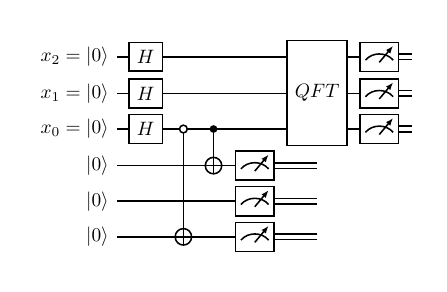
\begin{tikzpicture}
\node[scale=0.7]{    
\begin{quantikz}[row sep=0.005cm,column sep=0.22cm]
\lstick{$x_2 = \ket{0}$} & \gate{H}& \qw & \qw 
      & \qw & \gate[wires=3][0.5cm]{QFT} & \meter{} & \cw \\
\lstick{$x_1 = \ket{0}$} & \gate{H} & \qw & \qw       
      & \qw & & \meter{} & \cw \\
\lstick{$x_0 = \ket{0}$} & \gate{H} & \octrl{3} & \ctrl{1}
      & \qw & & \meter{} & \cw \\
\lstick{$\ket{0}$} & \qw & \qw & \targ{}
      & \meter{} & \cw \\
\lstick{$\ket{0}$} & \qw & \qw  & \qw
      & \meter{} & \cw \\
\lstick{$\ket{0}$} & \qw & \targ{} & \qw 
      & \meter{} & \cw
\end{quantikz}
};\end{tikzpicture}
\end{center}
\caption{\label{fig:shor15}Finding the period of $4^x \mod{15}$}
\end{wrapfigure}
\paragraph*{Easy Instances of Shor.}
The circuit in Fig.~\ref{fig:shor15} uses a hand-optimized
implementation of the modular exponentiation $4^x \mod{15}$ to factor
15 using Shor's algorithm. In a conventional forward execution, the
state before the QFT block is:
\[
\frac{1}{2\sqrt{2}} (
  (\ket{0} + \ket{2} + \ket{4} + \ket{6}) \ket{1} + 
  (\ket{1} + \ket{3} + \ket{5} + \ket{7}) \ket{4}
  )
\]
At this point, the ancilla register is measured to either $\ket{1}$ or
$\ket{4}$. In either case, the computational register snaps to a state
of the form $\sum_{r=0}^3 \ket{a+2r}$ whose QFT has peaks at $\ket{0}$
or $\ket{4}$ making them the most likely outcomes of measurements of
the computational register. If we measure $\ket{0}$, we repeat the
experiment; otherwise we infer that the period is~2.

In the retrodictive execution, we can start with the state
$\ket{x_2x_1x_0001}$ since 1 is guaranteed to be a possible
ancilla measurement. The first \cx-gate changes the state to
$\ket{x_2x_1x_0x_001}$ and the second \cx-gate produces
$\ket{x_2x_1x_0x_00x_0}$. At that point, we reconcile the
retrodictive result of the ancilla register $\ket{x_00x_0}$ with the
initial condition $\ket{000}$ to conclude that $x_0=0$. In other
words, in order to observe the ancilla at $001$, the computational
register must be initialized to a superposition of the form
$\ket{??0}$ where the least significant bit must be 0 and the other
two bits are unconstrained. Expanding the possibilities, the first
register needs to be in a superposition of the states $\ket{000},
\ket{010}, \ket{100}$ or $\ket{110}$ and we have just inferred using
purely classical but retrodictive reasoning that the period is
2. Significantly, this approach is robust and does not require small
hand-optimized circuits. Indeed, following the methods for producing
quantum circuits for arithmetic operations from first principles using
adders and multipliers~\cite{PhysRevA.54.147}, our implementation for
a general circuit for $a^x \mod{15}$ has 56538 generalized Toffoli
gates over 9 qubits, and yet the equations resulting from the
retrodictive execution in Fig.~\ref{fig:shor-eqs} are trivial and
immediately solvable as they only involve either the least significant
bit $x_0$ (when $a \in \{4,11,14\}$) or the least significant two bits
$x_0$ and $x_1$ (when $a \in \{2,7,8,13\}$). When the solution is
$x_0=0$, the period is 2. When the solution is $x_0=0,x_1=0$, the
period is 4.

\begin{figure}
\[\begin{array}{l@{\quad}llll@{~|~}l}
a=11 & x_0 = 0 &&&& x_0 = 0 \\
a=4,14 & 1 \oplus x_0 = 1 & x_0 = 0 &&
  & x_0 = 0 \\
a=7,13 & 1 \oplus x_1 \oplus x_0x_1 = 1 & x_0x_1 = 0 & x_0 \oplus x_1 \oplus x_0x_1 = 0 &  x_0 \oplus x_0x_1 = 0 & x_0=0, x_1=0 \\
a=2,8 & 1 \oplus x_0 \oplus x_1 \oplus x_0x_1 = 1 & x_0x_1 = 0 & x_1 \oplus x_0x_1 = 0 & x_0 \oplus x_0x_1 = 0  & x_0=0,x_1=0
\end{array}\]
\caption{\label{fig:shor-eqs}Equations generated by retrodictive
  execution of $a^x \mod{15}$ starting from observed result 1 and
  unknown $x_8x_7x_6x_5x_4x_3x_2x_1x_0$. The solution for the unknown
  variables is given in the last column.}
\end{figure}

\todo{
retroShor 51
n=12; a=49

Generalized Toffoli Gates with 3 controls = 8788
Generalized Toffoli Gates with 2 controls = 86866
Generalized Toffoli Gates with 1 controls = 81796

$1 \oplus x_2 \oplus x_0x_2 = 1$

$x_0x_1 \oplus x_0x_2 = 0$

$x_1 \oplus x_0x_1 = 0$

$x_0 \oplus x_1 \oplus x_1x_2 \oplus x_0x_1x_2 = 0$

$x_0 \oplus x_2 \oplus x_1x_2 = 0$

$x_0x_2 = 0$

----

$x_0=x_1=x_2=0$; period = 8
}

\todo{
retroShor 85
n=13; a=57

Generalized Toffoli Gates with 3 controls = 10976
Generalized Toffoli Gates with 2 controls = 109368
Generalized Toffoli Gates with 1 controls = 102704

$1 \oplus x_0x_1x_2 \oplus x_0x_1x_2x_3 \oplus x_1x_2x_3 \oplus x_1x_3 \oplus x_2x_3 \oplus x_3 = 1$

$x_0 \oplus x_0x_1x_2 \oplus x_0x_1x_2x_3 \oplus x_0x_2 \oplus x_0x_3 \oplus x_1x_3 = 0$

$x_0x_1x_2 \oplus x_0x_1x_3 \oplus x_1x_2x_3 \oplus x_2x_3 = 0$

$x_0x_1x_2x_3 \oplus x_0x_1x_3 \oplus x_0x_2 \oplus x_1 \oplus x_1x_2 = 0$

$x_0x_1 \oplus x_0x_1x_2x_3 \oplus x_0x_2 \oplus x_0x_2x_3 \oplus x_2 \oplus x_2x_3 \oplus x_3 = 0$

$x_0x_3 \oplus x_1x_2 \oplus x_1x_3 = 0$

$x_1x_2 \oplus x_1x_2x_3 \oplus x_2 \oplus x_2x_3 = 0$

period = 16
}

\todo{

retroShor 771
n=20; a=769

Generalized Toffoli Gates with 3 controls = 37044
Generalized Toffoli Gates with 2 controls = 381906
Generalized Toffoli Gates with 1 controls = 354564

$1 \oplus x_0x_3 \oplus x_3 = 1$

$x_0x_1x_2 \oplus x_0x_3 = 0$

$x_0x_1x_2 \oplus x_1x_2 = 0$

$x_0x_1x_2x_3 \oplus x_0x_2 \oplus x_1x_2 \oplus x_1x_2x_3 = 0$

$x_0x_2 \oplus x_0x_2x_3 \oplus x_1x_2x_3 \oplus x_2 = 0$

$x_0x_1 \oplus x_0x_1x_2 \oplus x_0x_1x_2x_3 \oplus x_0x_2 \oplus x_2 \oplus x_2x_3 = 0$

$x_0x_1 \oplus x_0x_1x_2 \oplus x_0x_1x_3 \oplus x_0x_2 \oplus x_1 \oplus x_1x_2 \oplus x_2 \oplus x_2x_3 = 0$

$x_0 \oplus x_0x_1x_2x_3 \oplus x_1 \oplus x_1x_2 \oplus x_1x_2x_3 \oplus x_1x_3 \oplus x_2 \oplus x_2x_3 = 0$

$x_0 \oplus x_0x_1x_3 \oplus x_0x_2x_3 \oplus x_1x_2x_3 \oplus x_1x_3 \oplus x_2x_3 \oplus x_3 = 0$

$x_0x_3 = 0$

period = 16
}

\todo{ longest clause gives period; basically we have constraints on
  all the vars in the longest clause; $2^i$ where i is the index of
  the next variable is the period

Try: 1285, 196611, 327685
}

\todo{

  Known Fermat primes: 3, 5, 17, 257, 65537

  some equations are bigger; these are sweet

  is it ever the case that we have an even number of clauses that are 1 in
  the formula for Shor

  it should $a^x mod N = 1$ for two different $x$ ???

}

\paragraph*{Shor 21.} 
The examples presented so far demonstrate that some instances of
quantum algorithms can be solved via classical symbolic retrodictive
execution. But as was already apparent in some examples (e.g. Grover),
running retrodictive execution may produce large residual equations
that are difficult to solve. To appreciate how large these equations
may be, we include the full set of equations produced for a
retrodictive execution of Shor's algorithm for factoring 21. Unlike
the number 15 which corresponds to a rare occurrence of products of
Fermat primes producing a period that is a power of 2 and hence
trivial to represent by equations of binary numbers, the period of 21
is not easily representable as a system of equations over binary
numbers. The equations which span about five pages in
Sec.~\ref{par:shor21} glaringly show the limitations of the basic
retrodictive execution approach and the need for additional insights.

%% I know 00000 is a solution because we picked ancilla = 1
%% solutions
%%
%% 00011, 00110,
%% 01001, 01100,
%% 11011, 10010, 10101,
%% 11000, 11011, 11110

%% Want the next smallest solution

%% x4 x3 x2 x1 x0
%%  0  0  0  1  1

n=4

\[\begin{array}{l}
1  \oplus x_0 
\oplus x_2
\oplus x_4 \\
~~
\oplus x_0x_2 
\oplus x_0x_3 
\oplus x_0x_4
\oplus x_2x_3 
\oplus x_2x_4
\oplus x_3x_4 \\
~~
\oplus x_0x_2x_4 \\
~~
\oplus x_0x_2x_3x_4 
= 1
\\[2ex]
x_0 
\oplus x_2
\oplus x_4  \\
~~
\oplus x_0x_3
\oplus x_2x_3
\oplus x_3x_4 \\
~~
\oplus x_0x_2x_3 
\oplus x_0x_3x_4 
\oplus x_2x_3x_4 \\
~~
\oplus x_0x_2x_3x_4 
= 0
\end{array}\]

n=5
\[\begin{array}{l}
1 \oplus x_0
\oplus x_2
\oplus x_3
\oplus x_4
\oplus x_5 \\
~~
\oplus x_0x_2
\oplus x_0x_4
\oplus x_2x_4
\oplus x_3x_5 \\
~~
\oplus x_0x_2x_3
\oplus x_0x_2x_5
\oplus x_0x_3x_4
\oplus x_0x_3x_5
\oplus x_0x_4x_5
\oplus x_2x_3x_4
\oplus x_2x_3x_5
\oplus x_2x_4x_5
\oplus x_3x_4x_5 \\
~~
\oplus x_0x_2x_3x_4
\oplus x_0x_2x_4x_5 \\
~~
\oplus x_0x_2x_3x_4x_5
= 1
\\[2ex]

x_0 
\oplus x_2
\oplus x_4 \\
~~
\oplus x_0x_3
\oplus x_0x_5
\oplus x_2x_3 
\oplus x_2x_5 
\oplus x_3x_4 
\oplus x_3x_5 
\oplus x_4x_5 \\
~~
\oplus x_0x_2x_3 
\oplus x_0x_2x_4 
\oplus x_0x_2x_5 
\oplus x_0x_3x_4 
\oplus x_0x_4x_5 
\oplus x_2x_3x_4 
\oplus x_2x_4x_5 \\
~~
\oplus x_0x_2x_3x_5
\oplus x_0x_3x_4x_5 
\oplus x_2x_3x_4x_5 \\
~~
\oplus x_0x_2x_3x_4x_5 
= 0
\\[2ex]

x_3
\oplus x_5 \\
~~
\oplus x_0x_2 
\oplus x_0x_3 
\oplus x_0x_4 
\oplus x_0x_5 
\oplus x_2x_3 
\oplus x_2x_4
\oplus x_2x_5
\oplus x_3x_4
\oplus x_4x_5 \\
~~
\oplus x_0x_2x_4 
\oplus x_0x_3x_5
\oplus x_2x_3x_5 
\oplus x_3x_4x_5 \\
~~
\oplus x_0x_2x_3x_4 
\oplus x_0x_2x_3x_5
\oplus x_0x_2x_4x_5 
\oplus x_0x_3x_4x_5 
\oplus x_2x_3x_4x_5
= 0
\end{array}\]

z-gate entanglement uses xor perhaps look at various patterns of
entanglement and how they are expressed in ANF then look at ANF and
how various properties are apparent without actually solving the
equations

n=6
\[\begin{array}{l}
1 \oplus x_0 \oplus x_2 \oplus x_3 \oplus x_4 \oplus x_5 \oplus x_6 \\
\oplus x_0x_2
\oplus x_0x_4 
\oplus x_0x_6
\oplus x_2x_4 
\oplus x_2x_6 
\oplus x_3x_5 
\oplus x_4x_6 \\
\oplus x_0x_2x_3
\oplus x_0x_2x_5 
\oplus x_0x_3x_4 
\oplus x_0x_3x_5 
\oplus x_0x_3x_6 
\oplus x_0x_4x_5
\oplus x_0x_5x_6
\oplus x_2x_3x_4 
\oplus x_2x_3x_5 
\oplus x_2x_3x_6 \\
~~\oplus x_2x_4x_5 
\oplus x_2x_5x_6 
\oplus x_3x_4x_5 
\oplus x_3x_4x_6 
\oplus x_3x_5x_6 
\oplus x_4x_5x_6 \\
\oplus x_0x_2x_3x_4 
\oplus x_0x_2x_3x_6 
\oplus x_0x_2x_4x_5 
\oplus x_0x_2x_4x_6 
\oplus x_0x_2x_5x_6 
\oplus x_0x_3x_4x_6
\oplus x_0x_4x_5x_6 
\oplus x_2x_3x_4x_6 
\oplus x_2x_4x_5x_6 \\
\oplus x_0x_2x_3x_4x_5 
\oplus x_0x_3x_4x_5x_6 
\oplus x_0x_2x_3x_5x_6
\oplus x_2x_3x_4x_5x_6 \\
\oplus x_0x_2x_3x_4x_5x_6 
= 1
\\[2ex]

x_0 
\oplus x_0x_2x_3 
\oplus x_0x_2x_3x_4x_5 
\oplus x_0x_2x_3x_4x_6 
\oplus x_0x_2x_3x_5 
\oplus x_0x_2x_3x_5x_6 
\oplus x_0x_2x_4 
\oplus x_0x_2x_4x_5x_6 
\oplus x_0x_2x_4x_6 
\oplus x_0x_2x_5 
\oplus x_0x_2x_6 
\oplus x_0x_3 
\oplus x_0x_3x_4 
\oplus x_0x_3x_4x_5 
\oplus x_0x_3x_4x_5x_6 
\oplus x_0x_3x_5x_6 
\oplus x_0x_3x_6 
\oplus x_0x_4x_5 
\oplus x_0x_4x_6 
\oplus x_0x_5 
\oplus x_0x_5x_6 
\oplus x_2 
\oplus x_2x_3 
\oplus x_2x_3x_4 
\oplus x_2x_3x_4x_5 
\oplus x_2x_3x_4x_5x_6 
\oplus x_2x_3x_5x_6 
\oplus x_2x_3x_6 
\oplus x_2x_4x_5 
\oplus x_2x_4x_6 
\oplus x_2x_5 
\oplus x_2x_5x_6 
\oplus x_3x_4 
\oplus x_3x_4x_5x_6 
\oplus x_3x_4x_6 
\oplus x_3x_5 
\oplus x_3x_6 
\oplus x_4 
\oplus x_4x_5 
\oplus x_4x_5x_6 
\oplus x_5x_6 
\oplus x_6 
= 0

\\[2ex]

x_0x_2 
\oplus x_0x_2x_3x_4 
\oplus x_0x_2x_3x_4x_5x_6 
\oplus x_0x_2x_3x_4x_6 
\oplus x_0x_2x_3x_5 
\oplus x_0x_2x_3x_6 
\oplus x_0x_2x_4 
\oplus x_0x_2x_4x_5 
\oplus x_0x_2x_4x_5x_6 
\oplus x_0x_2x_5x_6 
\oplus x_0x_2x_6 
\oplus x_0x_3 
\oplus x_0x_3x_4x_5 
\oplus x_0x_3x_4x_6 
\oplus x_0x_3x_5 
\oplus x_0x_3x_5x_6 
\oplus x_0x_4 
\oplus x_0x_4x_5x_6 
\oplus x_0x_4x_6 
\oplus x_0x_5 
\oplus x_0x_6 
\oplus x_2x_3 
\oplus x_2x_3x_4x_5 
\oplus x_2x_3x_4x_6 
\oplus x_2x_3x_5 
\oplus x_2x_3x_5x_6 
\oplus x_2x_4 
\oplus x_2x_4x_5x_6 
\oplus x_2x_4x_6 
\oplus x_2x_5 
\oplus x_2x_6 
\oplus x_3 
\oplus x_3x_4 
\oplus x_3x_4x_5 
\oplus x_3x_4x_5x_6 
\oplus x_3x_5x_6 
\oplus x_3x_6 
\oplus x_4x_5 
\oplus x_4x_6 
\oplus x_5 
\oplus x_5x_6 
= 0

\end{array}\]


\begin{wrapfigure}{r}{5cm}
\begin{center}
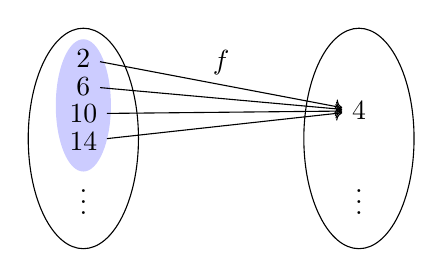
\begin{tikzpicture}[scale=0.7]
\draw (0,0) ellipse (1cm and 2cm);
\draw (5,0) circle (1cm and 2cm);
\fill[blue!20!white] (0,0.6) ellipse (0.5cm and 1.2cm);
\node (a) at (0,1.45) {2};
\node (b) at (0,0.95) {6};
\node (c) at (0,0.45) {10};
\node (d) at (0,-0.05) {14};
\node (t) at (5,0.5) {4};
\node at (0,-1) {$\vdots$};
\node at (5,-1) {$\vdots$};
\draw[->] (a) to node [above] {$f$} (t);
\draw[->] (b) -- (t);
\draw[->] (c) -- (t);
\draw[->] (d) -- (t);
\end{tikzpicture}
\end{center}
\caption{\label{fig:preimage}The pre-image of 4 under $f(x) = 7^x \mod 15$.}
\end{wrapfigure}
\paragraph*{Retrodictive Executions and Function Pre-images.}
Given finite sets $A$ and $B$, a function $f : A \rightarrow B$ and an
element $y \in B$, we define $\preim{f}{y}$, the pre-image of~$y$
under~$f$, as the set $\{ x \in A ~|~ f(x) = y \}$. For example, let
$A = B = \finset{2^4}$ and let $f(x) = 7^x \mod 15$, then the
collection of values that $f$ maps to~4, $\preim{f}{4}$, is the set
$\{ 2, 6, 10, 14 \}$ as shown in Fig.~\ref{fig:preimage}. Symbolic
retrodictive execution can be seen as a method to generate boolean
formulae that describe the pre-image of the function $f$ under
study. For the example in Fig.~\ref{fig:preimage}, retrodictive
execution might generate the formulae $x_1=1$ and $x_0=0$. The
(trivial in this case) solution for the formulae is indeed the set $\{
2, 6, 10, 14 \}$. The critical points to note, however, are that: (i)
solving the equations describing the pre-image is in general an
intractable (even for quantum computers) $\mathit{NP}$-complete
problem, and (ii) solving the equations is not needed for the quantum
algorithms in the previous section. \emph{Only some global properties
  of the pre-image are needed!} Indeed, we have already seen that for
solving the Deutsch-Jozsa problem, the only thing needed was whether
the formula contains some variables. Also for the Bernstein-Vazirani
problem, the only thing needed was the indices of the variables
occurring in the formula. For Grover's algorithm, we only need to
extract the singleton element in the pre-image and for Shor's
algorithm we only need to extract the periodicity of the elements in
the pre-image but retrodictive execution as presented so far is only
able to de-quantize some rare instances of algorithms.

\todo{
do communication protocols too ?

extensional vs intensional reasoning about functions

graph state: H,H,CZ
00   00
01   01
10   10
11 -11

check if H commutes with x and cx and ccx
so we only need H at beginning and end

insight: QFT insensitive to
0+2+4... vs 1+3+5...
so insensitive to where lsb is 0/1
so we only need to know if a variable is constant or varying 
fourier transform classical efficient in some cases

Kochen-Specker; interactive QM; observer free will; choice backtracks

universe uses lazy evaluation?

algebra of Toffoli and Hadamard
ZX calculus

values going at different speeds; intervals ideas; path types

\url{https://quantumalgorithmzoo.org}

$\ket{-}$; two classes of vars; +vars and -vars;
-vars infect +vars in control gates;
We have two operations +red (add red) -red (remove red)
Remember cx(+,-) = (-,-)
Some interactions (Toffoli) want to create more refined operations +/-(1/2)(red) +/-(red)
The more you do these operations the more precise it wants to be
  +/-(1/4)(red) +/-(1/2) red +/-(red)
taint analysis with increasing precisions; truncate at desired precision
(more and more colors)
The taint analysis groups variables in “waves” (superpositions) of
things that have the same color so the values we propagate are
“red: phase=p; frequency=f; involved variables={x1,x2,…}”

Possibility that collapse of wave function is information flow back
from measured future to present unknown initial conditions and then
back to rest of wave that was not measured

We need to explain ideas about time-reversal, prediction and retrodiction in 
physics. The laws of computation and the laws of physics are intimately related. 
When does knowing something about the future help us unveil the structure or 
symmetries of the past? It is like a detective story, but one with 
ramifications in complexity and/or efficiency. Problems involving questions 
where answers demand a Many(past)-to-one(future) map are at the root of 
our proposal

Possibility that collapse of wave function is information flow back
from measured future to present unknown initial conditions and then
back to rest of wave that was not measured

transactional interpretation?

instead of generating one formula; generating many formulas with
different weights or with various patterns of negative weights...
and sum them to get the patterns we need

\begin{itemize}
\item Symbolic (retrodictive) evaluation as a broader perspective to classical computation
\item Symbolic execution allows you to express/discover interference via shared variables
\item When interference pattern is simple symbolic execution reveals
  solutions faster (and completely classically)
\item Symbolic execution as a ``classical waves'' computing paradigm
\end{itemize}

Shor: have some fixed set of periodic states and always match the
closest one after each gate??

Sort clauses by length; the difference two consecutive clauses is the period !!!!!!

}

something has to give: either more entanglement requires more energy;
or signal back in time can be detected; or more mass

quantum algorithms built complex wavevfunction and then ask an
aggregate question; similar to molecules moving this way and that way
and then asking a question about temperature. It can be calculated by
average; no need to track every molecule.

but the program and the programming language is designed to track
every molecule; and then the observation is something aggregate and
statistical. Strange


Average frequency of each bit weighed by $2^i$. Run with one symbolic
variable and all others 0 to find contribution of this bit to
frequency or its average frquency.

Use qutrits for Shor 21. Equations should be nice

Then see if we can run with a parameter p for the base. Then we can
choose p dynamically. Perhaps keep a range of ``good'' values of p as
we execute.

%%%%%%%%%%%%%%%%%%%%%%%%%%%%%%%%%%%%%%%%%%%%%%%%%%%%%%%%%%%%%%%%%%%%%%%%%%%%%%%%%%%%%%%%%%

\printbibliography[heading=subbibliography]
\end{refsection}

%%%%%%%%%%%%%%%%%%%%%%%%%%%%%%%%%%%%%%%%%%%%%%%%%%%%%%%%%%%%%%%%%%%%%%%%%%%%%%%%%%%%%%%%%%

\begin{refsection}
\section{Methods}

\begin{quote}
You can’t connect the dots looking forward; you can only connect them
looking backwards.  So you have to trust that the dots will somehow
connect in your future. \emph{Steve Jobs}
\end{quote}

\paragraph*{Lazy Evaluation.}
Consider a program that searches for three different numbers $x$, $y$,
and $z$ each in the range $[1..n]$ and that sum to $s$. A
well-established design principle for solving such problems is the
\emph{generate-and-test} computational paradigm. Following this
principle, a simple program to solve this problem in the programming
language Haskell is:

\begin{verbatim}
generate :: Int -> [(Int,Int,Int)]
generate n =  [(x,y,z) | x <- [1..n], y <- [1..n], z <- [1..n]]

test :: Int -> [(Int,Int,Int)] -> [(Int,Int,Int)]
test s nums = [(x,y,z) | (x,y,z) <- nums, x /= y, x /= z, y /= z, x+y+z == s]

find :: Int -> Int -> (Int,Int,Int)
find s =  head . test s . generate
\end{verbatim}

The program consists of three functions: \verb|generate| that produces
all triples \verb|(x,y,z)| from \verb|(1,1,1)| to \verb|(n,n,n)|;
\verb|test| that checks that the numbers are different and that their
sum is equal to \verb|s|; and \verb|find| that composes the two
functions: generating all triples, testing the ones that satisfy the
condition, and returning the first solution. Running this program to
find numbers in the range $[1..6]$ that sum to 15 immediately produces
$(4,5,6)$ as expected.

But what if the range of interest was $[1..10000000]$ ? A na\"\i ve
execution of the generate-and-test method would be prohibitively
expensive as it would spend all its time generating an enormous number
of triples that are un-needed. Lazy demand-driven evaluation as
implemented in Haskell succeeds in a few seconds with the result
$(1,2,12)$, however. The idea is simple: instead of eagerly generating
all the triples, generate a process that, when queried, produces one
triple at a time on demand. Conceptually the execution starts from the
observer site which is asking for the first element of a list; this
demand is propagated to the function \verb|test| which itself
propagates the demand to the function \verb|generate|. As each triple
is generated, it is tested until one triple passes the test. This
triple is immediately returned without having to generate any
additional values.

\paragraph*{Partial Evaluation.}
Below is a Haskell program that computes $a^n$ by repeated squaring:
\begin{verbatim}
power :: Int -> Int -> Int
power a n
  | n == 0     = 1
  | n == 1     = a
  | even n     = let r = power a (n `div` 2) in r * r 
  | otherwise  = a * power a (n-1)
\end{verbatim}
When both inputs are known, e.g., \verb|a = 3| and \verb|n = 5|, the
program evaluates as follows:
\begin{verbatim}
   power 3 5
=  3 * power 3 4
=  3 * (let r1 = power 3 2 in r1 * r1)
=  3 * (let r1 = (let r2 = power 3 1 in r2 * r2) in r1 * r1)
=  3 * (let r1 = (let r2 = 3 in r2 * r2) in r1 * r1)
=  3 * (let r1 = 9 in r1 * r1)
=  243
\end{verbatim}

Partial evaluation is used when we only have partial information about
the inputs. Say we only know $n=5$. A partial evaluator then attempts
to evaluate \verb|power| with symbolic input \verb|a| and actual input
\verb|n=5|. This evaluation proceeds as follows:
\begin{verbatim}
   power a 5 
=  a * power a 4 
=  a * (let r1 = power a 2 in r1 * r1)
=  a * (let r1 = (let r2 = power a 1 in r2 * r2) in r1 * r1)
=  a * (let r1 = (let r2 = a in r2 * r2) in r1 * r1)
=  a * (let r1 = a * a in r1 * r1)
=  let r1 = a * a in a * r1 * r1
\end{verbatim}
All of this evaluation, simplification, and specialization happens
without knowledge of \verb|a|. Just knowing \verb|n| was enough to
produce a residual program that is much simpler. 

The evolution of a quantum system is typically understood as
proceeding forwards in time --- from the present to the future. As
shown in Fig.~\ref{fig:templateQC}(a), 

Since the conventional execution starts with complete ignorance about
the future, the initial state is prepared as a superposition that
includes every possibility. In a well-designed algorithm, , by the
time the computation reaches the measurement stages, the relative
phases and probability amplitudes in that enormous superposition have
become biased towards states of interest which are projected to
produce the final answer.

\paragraph*{Algebraic Normal Form (ANF).}
\label{para:anf}

~

\todo{
circuits have generalized toffoli gates: semantics (and of controls;
xor with target); ANF uses exactly those two primitives; explain

The resulting
expressions are in algebraic normal form~\cite{TOKAREVA20151} where
$+$ denotes exclusive-or. 

instances with no 'and' easy to solve

if only x and cx then symbolic execution is efficient; no need for last batch of H

can solve problem classically

connect with Gottsman-Knill
}

\paragraph*{Function Pre-Images and $\mathit{NP}$-Complete Problems.}
To appreciate the difficulty of computing pre-images in general, note
that finding the pre-image of a function subsumes several challenging
computational problems such as pre-image attacks on hash
functions~\cite{10.1007/978-3-540-25937-4_24}, predicting
environmental conditions that allow certain reactions to take place in
computational biology~\cite{Klotz2013,akutsu2009analyses}, and finding
the pre-image of feature vectors in the space induced by a kernel in
neural networks~\cite{1353287}. More to the point, the boolean
satisfiability problem SAT is expressible as a boolean function over
the input variables and solving a SAT problem is asking for the
pre-image of \textsf{true}. Indeed, based on the conjectured existence
of one-way functions which itself implies $\mathit{P} \neq
\mathit{NP}$, all these pre-images calculations are believed to be
computationally intractable in their most general setting.

\paragraph*{Complexity Analysis.}

~

\todo{ one pass over circuit BUT size of circuit may be exponential
  and complexity of normalizing to ANF not trivial
}

\paragraph*{Discussion.}

~

\todo{

observer 1 measures wires a,b; obs2 measures wires b,c; not commuting;
each obs gives partial solution to equations; but partial solutions
cannot lead to a global solution
 
KS suggests that equations do not have unique solutions; only
materialize when you measure;

can associate a probability with each variable in a equation: look at
all solutions and see the contribution of each variable to these
solutions.

}

\paragraph*{Data Availability.}
All execution results will be made available and can be replicated by
executing the associated software.

\paragraph*{Code Availability.}
The computer programs used to generate the circuits and symbolically
execute the quantum algorithms retrodictively will be made publicly
available.

\paragraph*{Author Contributions.}
The idea of symbolic evaluation is due to A.S. The connection to
retrodictive quantum mechanics is due to G.O. The connection to
partial evaluation is due to J.C. Both A.S. and J.C. contributed to
the software code to run the experiments. Both A.S. and
G.O. contributed to the analysis of the quantum algorithms and their
de-quantization. All authors contributed to the writing of the
document.

\paragraph*{Competing Interests.}
No competing interests.

\paragraph*{Materials \& Correspondence.}
The corresponding author is Gerardo Ortiz. 

\paragraph*{Supplementary Information.} 
\label{par:shor21}

Equations generated by retrodictive execution of $16^x \mod{21}$
starting from observed result 1 and unknown $x$. The circuit consists
of 9 qubits, 36400 \cx-gates, 38200 \ccx-gates, and 4000
\cccx-gates. There are only three equations but each equation is
exponentially large.

$1 \oplus x_0 \oplus x_0x_1x_2 \oplus x_0x_1x_2x_3x_4 \oplus x_0x_1x_2x_3x_4x_5x_6 \oplus x_0x_1x_2x_3x_4x_5x_6x_7x_8 \oplus x_0x_1x_2x_3x_4x_5x_6x_7x_9 \oplus x_0x_1x_2x_3x_4x_5x_6x_8 \oplus x_0x_1x_2x_3x_4x_5x_6x_8x_9 \oplus x_0x_1x_2x_3x_4x_5x_7 \oplus x_0x_1x_2x_3x_4x_5x_7x_8x_9 \oplus x_0x_1x_2x_3x_4x_5x_7x_9 \oplus x_0x_1x_2x_3x_4x_5x_8 \oplus x_0x_1x_2x_3x_4x_5x_9 \oplus x_0x_1x_2x_3x_4x_6 \oplus x_0x_1x_2x_3x_4x_6x_7 \oplus x_0x_1x_2x_3x_4x_6x_7x_8 \oplus x_0x_1x_2x_3x_4x_6x_7x_8x_9 \oplus x_0x_1x_2x_3x_4x_6x_8x_9 \oplus x_0x_1x_2x_3x_4x_6x_9 \oplus x_0x_1x_2x_3x_4x_7x_8 \oplus x_0x_1x_2x_3x_4x_7x_9 \oplus x_0x_1x_2x_3x_4x_8 \oplus x_0x_1x_2x_3x_4x_8x_9 \oplus x_0x_1x_2x_3x_5 \oplus x_0x_1x_2x_3x_5x_6x_7 \oplus x_0x_1x_2x_3x_5x_6x_7x_8x_9 \oplus x_0x_1x_2x_3x_5x_6x_7x_9 \oplus x_0x_1x_2x_3x_5x_6x_8 \oplus x_0x_1x_2x_3x_5x_6x_9 \oplus x_0x_1x_2x_3x_5x_7 \oplus x_0x_1x_2x_3x_5x_7x_8 \oplus x_0x_1x_2x_3x_5x_7x_8x_9 \oplus x_0x_1x_2x_3x_5x_8x_9 \oplus x_0x_1x_2x_3x_5x_9 \oplus x_0x_1x_2x_3x_6 \oplus x_0x_1x_2x_3x_6x_7x_8 \oplus x_0x_1x_2x_3x_6x_7x_9 \oplus x_0x_1x_2x_3x_6x_8 \oplus x_0x_1x_2x_3x_6x_8x_9 \oplus x_0x_1x_2x_3x_7 \oplus x_0x_1x_2x_3x_7x_8x_9 \oplus x_0x_1x_2x_3x_7x_9 \oplus x_0x_1x_2x_3x_8 \oplus x_0x_1x_2x_3x_9 \oplus x_0x_1x_2x_4 \oplus x_0x_1x_2x_4x_5 \oplus x_0x_1x_2x_4x_5x_6 \oplus x_0x_1x_2x_4x_5x_6x_7 \oplus x_0x_1x_2x_4x_5x_6x_7x_8 \oplus x_0x_1x_2x_4x_5x_6x_7x_8x_9 \oplus x_0x_1x_2x_4x_5x_6x_8x_9 \oplus x_0x_1x_2x_4x_5x_6x_9 \oplus x_0x_1x_2x_4x_5x_7x_8 \oplus x_0x_1x_2x_4x_5x_7x_9 \oplus x_0x_1x_2x_4x_5x_8 \oplus x_0x_1x_2x_4x_5x_8x_9 \oplus x_0x_1x_2x_4x_6x_7 \oplus x_0x_1x_2x_4x_6x_7x_8x_9 \oplus x_0x_1x_2x_4x_6x_7x_9 \oplus x_0x_1x_2x_4x_6x_8 \oplus x_0x_1x_2x_4x_6x_9 \oplus x_0x_1x_2x_4x_7 \oplus x_0x_1x_2x_4x_7x_8 \oplus x_0x_1x_2x_4x_7x_8x_9 \oplus x_0x_1x_2x_4x_8x_9 \oplus x_0x_1x_2x_4x_9 \oplus x_0x_1x_2x_5x_6 \oplus x_0x_1x_2x_5x_6x_7x_8 \oplus x_0x_1x_2x_5x_6x_7x_9 \oplus x_0x_1x_2x_5x_6x_8 \oplus x_0x_1x_2x_5x_6x_8x_9 \oplus x_0x_1x_2x_5x_7 \oplus x_0x_1x_2x_5x_7x_8x_9 \oplus x_0x_1x_2x_5x_7x_9 \oplus x_0x_1x_2x_5x_8 \oplus x_0x_1x_2x_5x_9 \oplus x_0x_1x_2x_6 \oplus x_0x_1x_2x_6x_7 \oplus x_0x_1x_2x_6x_7x_8 \oplus x_0x_1x_2x_6x_7x_8x_9 \oplus x_0x_1x_2x_6x_8x_9 \oplus x_0x_1x_2x_6x_9 \oplus x_0x_1x_2x_7x_8 \oplus x_0x_1x_2x_7x_9 \oplus x_0x_1x_2x_8 \oplus x_0x_1x_2x_8x_9 \oplus x_0x_1x_3 \oplus x_0x_1x_3x_4x_5 \oplus x_0x_1x_3x_4x_5x_6x_7 \oplus x_0x_1x_3x_4x_5x_6x_7x_8x_9 \oplus x_0x_1x_3x_4x_5x_6x_7x_9 \oplus x_0x_1x_3x_4x_5x_6x_8 \oplus x_0x_1x_3x_4x_5x_6x_9 \oplus x_0x_1x_3x_4x_5x_7 \oplus x_0x_1x_3x_4x_5x_7x_8 \oplus x_0x_1x_3x_4x_5x_7x_8x_9 \oplus x_0x_1x_3x_4x_5x_8x_9 \oplus x_0x_1x_3x_4x_5x_9 \oplus x_0x_1x_3x_4x_6 \oplus x_0x_1x_3x_4x_6x_7x_8 \oplus x_0x_1x_3x_4x_6x_7x_9 \oplus x_0x_1x_3x_4x_6x_8 \oplus x_0x_1x_3x_4x_6x_8x_9 \oplus x_0x_1x_3x_4x_7 \oplus x_0x_1x_3x_4x_7x_8x_9 \oplus x_0x_1x_3x_4x_7x_9 \oplus x_0x_1x_3x_4x_8 \oplus x_0x_1x_3x_4x_9 \oplus x_0x_1x_3x_5 \oplus x_0x_1x_3x_5x_6 \oplus x_0x_1x_3x_5x_6x_7 \oplus x_0x_1x_3x_5x_6x_7x_8 \oplus x_0x_1x_3x_5x_6x_7x_8x_9 \oplus x_0x_1x_3x_5x_6x_8x_9 \oplus x_0x_1x_3x_5x_6x_9 \oplus x_0x_1x_3x_5x_7x_8 \oplus x_0x_1x_3x_5x_7x_9 \oplus x_0x_1x_3x_5x_8 \oplus x_0x_1x_3x_5x_8x_9 \oplus x_0x_1x_3x_6x_7 \oplus x_0x_1x_3x_6x_7x_8x_9 \oplus x_0x_1x_3x_6x_7x_9 \oplus x_0x_1x_3x_6x_8 \oplus x_0x_1x_3x_6x_9 \oplus x_0x_1x_3x_7 \oplus x_0x_1x_3x_7x_8 \oplus x_0x_1x_3x_7x_8x_9 \oplus x_0x_1x_3x_8x_9 \oplus x_0x_1x_3x_9 \oplus x_0x_1x_4 \oplus x_0x_1x_4x_5x_6 \oplus x_0x_1x_4x_5x_6x_7x_8 \oplus x_0x_1x_4x_5x_6x_7x_9 \oplus x_0x_1x_4x_5x_6x_8 \oplus x_0x_1x_4x_5x_6x_8x_9 \oplus x_0x_1x_4x_5x_7 \oplus x_0x_1x_4x_5x_7x_8x_9 \oplus x_0x_1x_4x_5x_7x_9 \oplus x_0x_1x_4x_5x_8 \oplus x_0x_1x_4x_5x_9 \oplus x_0x_1x_4x_6 \oplus x_0x_1x_4x_6x_7 \oplus x_0x_1x_4x_6x_7x_8 \oplus x_0x_1x_4x_6x_7x_8x_9 \oplus x_0x_1x_4x_6x_8x_9 \oplus x_0x_1x_4x_6x_9 \oplus x_0x_1x_4x_7x_8 \oplus x_0x_1x_4x_7x_9 \oplus x_0x_1x_4x_8 \oplus x_0x_1x_4x_8x_9 \oplus x_0x_1x_5 \oplus x_0x_1x_5x_6x_7 \oplus x_0x_1x_5x_6x_7x_8x_9 \oplus x_0x_1x_5x_6x_7x_9 \oplus x_0x_1x_5x_6x_8 \oplus x_0x_1x_5x_6x_9 \oplus x_0x_1x_5x_7 \oplus x_0x_1x_5x_7x_8 \oplus x_0x_1x_5x_7x_8x_9 \oplus x_0x_1x_5x_8x_9 \oplus x_0x_1x_5x_9 \oplus x_0x_1x_6 \oplus x_0x_1x_6x_7x_8 \oplus x_0x_1x_6x_7x_9 \oplus x_0x_1x_6x_8 \oplus x_0x_1x_6x_8x_9 \oplus x_0x_1x_7 \oplus x_0x_1x_7x_8x_9 \oplus x_0x_1x_7x_9 \oplus x_0x_1x_8 \oplus x_0x_1x_9 \oplus x_0x_2 \oplus x_0x_2x_3 \oplus x_0x_2x_3x_4 \oplus x_0x_2x_3x_4x_5 \oplus x_0x_2x_3x_4x_5x_6 \oplus x_0x_2x_3x_4x_5x_6x_7 \oplus x_0x_2x_3x_4x_5x_6x_7x_8 \oplus x_0x_2x_3x_4x_5x_6x_7x_8x_9 \oplus x_0x_2x_3x_4x_5x_6x_8x_9 \oplus x_0x_2x_3x_4x_5x_6x_9 \oplus x_0x_2x_3x_4x_5x_7x_8 \oplus x_0x_2x_3x_4x_5x_7x_9 \oplus x_0x_2x_3x_4x_5x_8 \oplus x_0x_2x_3x_4x_5x_8x_9 \oplus x_0x_2x_3x_4x_6x_7 \oplus x_0x_2x_3x_4x_6x_7x_8x_9 \oplus x_0x_2x_3x_4x_6x_7x_9 \oplus x_0x_2x_3x_4x_6x_8 \oplus x_0x_2x_3x_4x_6x_9 \oplus x_0x_2x_3x_4x_7 \oplus x_0x_2x_3x_4x_7x_8 \oplus x_0x_2x_3x_4x_7x_8x_9 \oplus x_0x_2x_3x_4x_8x_9 \oplus x_0x_2x_3x_4x_9 \oplus x_0x_2x_3x_5x_6 \oplus x_0x_2x_3x_5x_6x_7x_8 \oplus x_0x_2x_3x_5x_6x_7x_9 \oplus x_0x_2x_3x_5x_6x_8 \oplus x_0x_2x_3x_5x_6x_8x_9 \oplus x_0x_2x_3x_5x_7 \oplus x_0x_2x_3x_5x_7x_8x_9 \oplus x_0x_2x_3x_5x_7x_9 \oplus x_0x_2x_3x_5x_8 \oplus x_0x_2x_3x_5x_9 \oplus x_0x_2x_3x_6 \oplus x_0x_2x_3x_6x_7 \oplus x_0x_2x_3x_6x_7x_8 \oplus x_0x_2x_3x_6x_7x_8x_9 \oplus x_0x_2x_3x_6x_8x_9 \oplus x_0x_2x_3x_6x_9 \oplus x_0x_2x_3x_7x_8 \oplus x_0x_2x_3x_7x_9 \oplus x_0x_2x_3x_8 \oplus x_0x_2x_3x_8x_9 \oplus x_0x_2x_4x_5 \oplus x_0x_2x_4x_5x_6x_7 \oplus x_0x_2x_4x_5x_6x_7x_8x_9 \oplus x_0x_2x_4x_5x_6x_7x_9 \oplus x_0x_2x_4x_5x_6x_8 \oplus x_0x_2x_4x_5x_6x_9 \oplus x_0x_2x_4x_5x_7 \oplus x_0x_2x_4x_5x_7x_8 \oplus x_0x_2x_4x_5x_7x_8x_9 \oplus x_0x_2x_4x_5x_8x_9 \oplus x_0x_2x_4x_5x_9 \oplus x_0x_2x_4x_6 \oplus x_0x_2x_4x_6x_7x_8 \oplus x_0x_2x_4x_6x_7x_9 \oplus x_0x_2x_4x_6x_8 \oplus x_0x_2x_4x_6x_8x_9 \oplus x_0x_2x_4x_7 \oplus x_0x_2x_4x_7x_8x_9 \oplus x_0x_2x_4x_7x_9 \oplus x_0x_2x_4x_8 \oplus x_0x_2x_4x_9 \oplus x_0x_2x_5 \oplus x_0x_2x_5x_6 \oplus x_0x_2x_5x_6x_7 \oplus x_0x_2x_5x_6x_7x_8 \oplus x_0x_2x_5x_6x_7x_8x_9 \oplus x_0x_2x_5x_6x_8x_9 \oplus x_0x_2x_5x_6x_9 \oplus x_0x_2x_5x_7x_8 \oplus x_0x_2x_5x_7x_9 \oplus x_0x_2x_5x_8 \oplus x_0x_2x_5x_8x_9 \oplus x_0x_2x_6x_7 \oplus x_0x_2x_6x_7x_8x_9 \oplus x_0x_2x_6x_7x_9 \oplus x_0x_2x_6x_8 \oplus x_0x_2x_6x_9 \oplus x_0x_2x_7 \oplus x_0x_2x_7x_8 \oplus x_0x_2x_7x_8x_9 \oplus x_0x_2x_8x_9 \oplus x_0x_2x_9 \oplus x_0x_3x_4 \oplus x_0x_3x_4x_5x_6 \oplus x_0x_3x_4x_5x_6x_7x_8 \oplus x_0x_3x_4x_5x_6x_7x_9 \oplus x_0x_3x_4x_5x_6x_8 \oplus x_0x_3x_4x_5x_6x_8x_9 \oplus x_0x_3x_4x_5x_7 \oplus x_0x_3x_4x_5x_7x_8x_9 \oplus x_0x_3x_4x_5x_7x_9 \oplus x_0x_3x_4x_5x_8 \oplus x_0x_3x_4x_5x_9 \oplus x_0x_3x_4x_6 \oplus x_0x_3x_4x_6x_7 \oplus x_0x_3x_4x_6x_7x_8 \oplus x_0x_3x_4x_6x_7x_8x_9 \oplus x_0x_3x_4x_6x_8x_9 \oplus x_0x_3x_4x_6x_9 \oplus x_0x_3x_4x_7x_8 \oplus x_0x_3x_4x_7x_9 \oplus x_0x_3x_4x_8 \oplus x_0x_3x_4x_8x_9 \oplus x_0x_3x_5 \oplus x_0x_3x_5x_6x_7 \oplus x_0x_3x_5x_6x_7x_8x_9 \oplus x_0x_3x_5x_6x_7x_9 \oplus x_0x_3x_5x_6x_8 \oplus x_0x_3x_5x_6x_9 \oplus x_0x_3x_5x_7 \oplus x_0x_3x_5x_7x_8 \oplus x_0x_3x_5x_7x_8x_9 \oplus x_0x_3x_5x_8x_9 \oplus x_0x_3x_5x_9 \oplus x_0x_3x_6 \oplus x_0x_3x_6x_7x_8 \oplus x_0x_3x_6x_7x_9 \oplus x_0x_3x_6x_8 \oplus x_0x_3x_6x_8x_9 \oplus x_0x_3x_7 \oplus x_0x_3x_7x_8x_9 \oplus x_0x_3x_7x_9 \oplus x_0x_3x_8 \oplus x_0x_3x_9 \oplus x_0x_4 \oplus x_0x_4x_5 \oplus x_0x_4x_5x_6 \oplus x_0x_4x_5x_6x_7 \oplus x_0x_4x_5x_6x_7x_8 \oplus x_0x_4x_5x_6x_7x_8x_9 \oplus x_0x_4x_5x_6x_8x_9 \oplus x_0x_4x_5x_6x_9 \oplus x_0x_4x_5x_7x_8 \oplus x_0x_4x_5x_7x_9 \oplus x_0x_4x_5x_8 \oplus x_0x_4x_5x_8x_9 \oplus x_0x_4x_6x_7 \oplus x_0x_4x_6x_7x_8x_9 \oplus x_0x_4x_6x_7x_9 \oplus x_0x_4x_6x_8 \oplus x_0x_4x_6x_9 \oplus x_0x_4x_7 \oplus x_0x_4x_7x_8 \oplus x_0x_4x_7x_8x_9 \oplus x_0x_4x_8x_9 \oplus x_0x_4x_9 \oplus x_0x_5x_6 \oplus x_0x_5x_6x_7x_8 \oplus x_0x_5x_6x_7x_9 \oplus x_0x_5x_6x_8 \oplus x_0x_5x_6x_8x_9 \oplus x_0x_5x_7 \oplus x_0x_5x_7x_8x_9 \oplus x_0x_5x_7x_9 \oplus x_0x_5x_8 \oplus x_0x_5x_9 \oplus x_0x_6 \oplus x_0x_6x_7 \oplus x_0x_6x_7x_8 \oplus x_0x_6x_7x_8x_9 \oplus x_0x_6x_8x_9 \oplus x_0x_6x_9 \oplus x_0x_7x_8 \oplus x_0x_7x_9 \oplus x_0x_8 \oplus x_0x_8x_9 \oplus x_1 \oplus x_1x_2x_3 \oplus x_1x_2x_3x_4x_5 \oplus x_1x_2x_3x_4x_5x_6x_7 \oplus x_1x_2x_3x_4x_5x_6x_7x_8x_9 \oplus x_1x_2x_3x_4x_5x_6x_7x_9 \oplus x_1x_2x_3x_4x_5x_6x_8 \oplus x_1x_2x_3x_4x_5x_6x_9 \oplus x_1x_2x_3x_4x_5x_7 \oplus x_1x_2x_3x_4x_5x_7x_8 \oplus x_1x_2x_3x_4x_5x_7x_8x_9 \oplus x_1x_2x_3x_4x_5x_8x_9 \oplus x_1x_2x_3x_4x_5x_9 \oplus x_1x_2x_3x_4x_6 \oplus x_1x_2x_3x_4x_6x_7x_8 \oplus x_1x_2x_3x_4x_6x_7x_9 \oplus x_1x_2x_3x_4x_6x_8 \oplus x_1x_2x_3x_4x_6x_8x_9 \oplus x_1x_2x_3x_4x_7 \oplus x_1x_2x_3x_4x_7x_8x_9 \oplus x_1x_2x_3x_4x_7x_9 \oplus x_1x_2x_3x_4x_8 \oplus x_1x_2x_3x_4x_9 \oplus x_1x_2x_3x_5 \oplus x_1x_2x_3x_5x_6 \oplus x_1x_2x_3x_5x_6x_7 \oplus x_1x_2x_3x_5x_6x_7x_8 \oplus x_1x_2x_3x_5x_6x_7x_8x_9 \oplus x_1x_2x_3x_5x_6x_8x_9 \oplus x_1x_2x_3x_5x_6x_9 \oplus x_1x_2x_3x_5x_7x_8 \oplus x_1x_2x_3x_5x_7x_9 \oplus x_1x_2x_3x_5x_8 \oplus x_1x_2x_3x_5x_8x_9 \oplus x_1x_2x_3x_6x_7 \oplus x_1x_2x_3x_6x_7x_8x_9 \oplus x_1x_2x_3x_6x_7x_9 \oplus x_1x_2x_3x_6x_8 \oplus x_1x_2x_3x_6x_9 \oplus x_1x_2x_3x_7 \oplus x_1x_2x_3x_7x_8 \oplus x_1x_2x_3x_7x_8x_9 \oplus x_1x_2x_3x_8x_9 \oplus x_1x_2x_3x_9 \oplus x_1x_2x_4 \oplus x_1x_2x_4x_5x_6 \oplus x_1x_2x_4x_5x_6x_7x_8 \oplus x_1x_2x_4x_5x_6x_7x_9 \oplus x_1x_2x_4x_5x_6x_8 \oplus x_1x_2x_4x_5x_6x_8x_9 \oplus x_1x_2x_4x_5x_7 \oplus x_1x_2x_4x_5x_7x_8x_9 \oplus x_1x_2x_4x_5x_7x_9 \oplus x_1x_2x_4x_5x_8 \oplus x_1x_2x_4x_5x_9 \oplus x_1x_2x_4x_6 \oplus x_1x_2x_4x_6x_7 \oplus x_1x_2x_4x_6x_7x_8 \oplus x_1x_2x_4x_6x_7x_8x_9 \oplus x_1x_2x_4x_6x_8x_9 \oplus x_1x_2x_4x_6x_9 \oplus x_1x_2x_4x_7x_8 \oplus x_1x_2x_4x_7x_9 \oplus x_1x_2x_4x_8 \oplus x_1x_2x_4x_8x_9 \oplus x_1x_2x_5 \oplus x_1x_2x_5x_6x_7 \oplus x_1x_2x_5x_6x_7x_8x_9 \oplus x_1x_2x_5x_6x_7x_9 \oplus x_1x_2x_5x_6x_8 \oplus x_1x_2x_5x_6x_9 \oplus x_1x_2x_5x_7 \oplus x_1x_2x_5x_7x_8 \oplus x_1x_2x_5x_7x_8x_9 \oplus x_1x_2x_5x_8x_9 \oplus x_1x_2x_5x_9 \oplus x_1x_2x_6 \oplus x_1x_2x_6x_7x_8 \oplus x_1x_2x_6x_7x_9 \oplus x_1x_2x_6x_8 \oplus x_1x_2x_6x_8x_9 \oplus x_1x_2x_7 \oplus x_1x_2x_7x_8x_9 \oplus x_1x_2x_7x_9 \oplus x_1x_2x_8 \oplus x_1x_2x_9 \oplus x_1x_3 \oplus x_1x_3x_4 \oplus x_1x_3x_4x_5 \oplus x_1x_3x_4x_5x_6 \oplus x_1x_3x_4x_5x_6x_7 \oplus x_1x_3x_4x_5x_6x_7x_8 \oplus x_1x_3x_4x_5x_6x_7x_8x_9 \oplus x_1x_3x_4x_5x_6x_8x_9 \oplus x_1x_3x_4x_5x_6x_9 \oplus x_1x_3x_4x_5x_7x_8 \oplus x_1x_3x_4x_5x_7x_9 \oplus x_1x_3x_4x_5x_8 \oplus x_1x_3x_4x_5x_8x_9 \oplus x_1x_3x_4x_6x_7 \oplus x_1x_3x_4x_6x_7x_8x_9 \oplus x_1x_3x_4x_6x_7x_9 \oplus x_1x_3x_4x_6x_8 \oplus x_1x_3x_4x_6x_9 \oplus x_1x_3x_4x_7 \oplus x_1x_3x_4x_7x_8 \oplus x_1x_3x_4x_7x_8x_9 \oplus x_1x_3x_4x_8x_9 \oplus x_1x_3x_4x_9 \oplus x_1x_3x_5x_6 \oplus x_1x_3x_5x_6x_7x_8 \oplus x_1x_3x_5x_6x_7x_9 \oplus x_1x_3x_5x_6x_8 \oplus x_1x_3x_5x_6x_8x_9 \oplus x_1x_3x_5x_7 \oplus x_1x_3x_5x_7x_8x_9 \oplus x_1x_3x_5x_7x_9 \oplus x_1x_3x_5x_8 \oplus x_1x_3x_5x_9 \oplus x_1x_3x_6 \oplus x_1x_3x_6x_7 \oplus x_1x_3x_6x_7x_8 \oplus x_1x_3x_6x_7x_8x_9 \oplus x_1x_3x_6x_8x_9 \oplus x_1x_3x_6x_9 \oplus x_1x_3x_7x_8 \oplus x_1x_3x_7x_9 \oplus x_1x_3x_8 \oplus x_1x_3x_8x_9 \oplus x_1x_4x_5 \oplus x_1x_4x_5x_6x_7 \oplus x_1x_4x_5x_6x_7x_8x_9 \oplus x_1x_4x_5x_6x_7x_9 \oplus x_1x_4x_5x_6x_8 \oplus x_1x_4x_5x_6x_9 \oplus x_1x_4x_5x_7 \oplus x_1x_4x_5x_7x_8 \oplus x_1x_4x_5x_7x_8x_9 \oplus x_1x_4x_5x_8x_9 \oplus x_1x_4x_5x_9 \oplus x_1x_4x_6 \oplus x_1x_4x_6x_7x_8 \oplus x_1x_4x_6x_7x_9 \oplus x_1x_4x_6x_8 \oplus x_1x_4x_6x_8x_9 \oplus x_1x_4x_7 \oplus x_1x_4x_7x_8x_9 \oplus x_1x_4x_7x_9 \oplus x_1x_4x_8 \oplus x_1x_4x_9 \oplus x_1x_5 \oplus x_1x_5x_6 \oplus x_1x_5x_6x_7 \oplus x_1x_5x_6x_7x_8 \oplus x_1x_5x_6x_7x_8x_9 \oplus x_1x_5x_6x_8x_9 \oplus x_1x_5x_6x_9 \oplus x_1x_5x_7x_8 \oplus x_1x_5x_7x_9 \oplus x_1x_5x_8 \oplus x_1x_5x_8x_9 \oplus x_1x_6x_7 \oplus x_1x_6x_7x_8x_9 \oplus x_1x_6x_7x_9 \oplus x_1x_6x_8 \oplus x_1x_6x_9 \oplus x_1x_7 \oplus x_1x_7x_8 \oplus x_1x_7x_8x_9 \oplus x_1x_8x_9 \oplus x_1x_9 \oplus x_2 \oplus x_2x_3x_4 \oplus x_2x_3x_4x_5x_6 \oplus x_2x_3x_4x_5x_6x_7x_8 \oplus x_2x_3x_4x_5x_6x_7x_9 \oplus x_2x_3x_4x_5x_6x_8 \oplus x_2x_3x_4x_5x_6x_8x_9 \oplus x_2x_3x_4x_5x_7 \oplus x_2x_3x_4x_5x_7x_8x_9 \oplus x_2x_3x_4x_5x_7x_9 \oplus x_2x_3x_4x_5x_8 \oplus x_2x_3x_4x_5x_9 \oplus x_2x_3x_4x_6 \oplus x_2x_3x_4x_6x_7 \oplus x_2x_3x_4x_6x_7x_8 \oplus x_2x_3x_4x_6x_7x_8x_9 \oplus x_2x_3x_4x_6x_8x_9 \oplus x_2x_3x_4x_6x_9 \oplus x_2x_3x_4x_7x_8 \oplus x_2x_3x_4x_7x_9 \oplus x_2x_3x_4x_8 \oplus x_2x_3x_4x_8x_9 \oplus x_2x_3x_5 \oplus x_2x_3x_5x_6x_7 \oplus x_2x_3x_5x_6x_7x_8x_9 \oplus x_2x_3x_5x_6x_7x_9 \oplus x_2x_3x_5x_6x_8 \oplus x_2x_3x_5x_6x_9 \oplus x_2x_3x_5x_7 \oplus x_2x_3x_5x_7x_8 \oplus x_2x_3x_5x_7x_8x_9 \oplus x_2x_3x_5x_8x_9 \oplus x_2x_3x_5x_9 \oplus x_2x_3x_6 \oplus x_2x_3x_6x_7x_8 \oplus x_2x_3x_6x_7x_9 \oplus x_2x_3x_6x_8 \oplus x_2x_3x_6x_8x_9 \oplus x_2x_3x_7 \oplus x_2x_3x_7x_8x_9 \oplus x_2x_3x_7x_9 \oplus x_2x_3x_8 \oplus x_2x_3x_9 \oplus x_2x_4 \oplus x_2x_4x_5 \oplus x_2x_4x_5x_6 \oplus x_2x_4x_5x_6x_7 \oplus x_2x_4x_5x_6x_7x_8 \oplus x_2x_4x_5x_6x_7x_8x_9 \oplus x_2x_4x_5x_6x_8x_9 \oplus x_2x_4x_5x_6x_9 \oplus x_2x_4x_5x_7x_8 \oplus x_2x_4x_5x_7x_9 \oplus x_2x_4x_5x_8 \oplus x_2x_4x_5x_8x_9 \oplus x_2x_4x_6x_7 \oplus x_2x_4x_6x_7x_8x_9 \oplus x_2x_4x_6x_7x_9 \oplus x_2x_4x_6x_8 \oplus x_2x_4x_6x_9 \oplus x_2x_4x_7 \oplus x_2x_4x_7x_8 \oplus x_2x_4x_7x_8x_9 \oplus x_2x_4x_8x_9 \oplus x_2x_4x_9 \oplus x_2x_5x_6 \oplus x_2x_5x_6x_7x_8 \oplus x_2x_5x_6x_7x_9 \oplus x_2x_5x_6x_8 \oplus x_2x_5x_6x_8x_9 \oplus x_2x_5x_7 \oplus x_2x_5x_7x_8x_9 \oplus x_2x_5x_7x_9 \oplus x_2x_5x_8 \oplus x_2x_5x_9 \oplus x_2x_6 \oplus x_2x_6x_7 \oplus x_2x_6x_7x_8 \oplus x_2x_6x_7x_8x_9 \oplus x_2x_6x_8x_9 \oplus x_2x_6x_9 \oplus x_2x_7x_8 \oplus x_2x_7x_9 \oplus x_2x_8 \oplus x_2x_8x_9 \oplus x_3 \oplus x_3x_4x_5 \oplus x_3x_4x_5x_6x_7 \oplus x_3x_4x_5x_6x_7x_8x_9 \oplus x_3x_4x_5x_6x_7x_9 \oplus x_3x_4x_5x_6x_8 \oplus x_3x_4x_5x_6x_9 \oplus x_3x_4x_5x_7 \oplus x_3x_4x_5x_7x_8 \oplus x_3x_4x_5x_7x_8x_9 \oplus x_3x_4x_5x_8x_9 \oplus x_3x_4x_5x_9 \oplus x_3x_4x_6 \oplus x_3x_4x_6x_7x_8 \oplus x_3x_4x_6x_7x_9 \oplus x_3x_4x_6x_8 \oplus x_3x_4x_6x_8x_9 \oplus x_3x_4x_7 \oplus x_3x_4x_7x_8x_9 \oplus x_3x_4x_7x_9 \oplus x_3x_4x_8 \oplus x_3x_4x_9 \oplus x_3x_5 \oplus x_3x_5x_6 \oplus x_3x_5x_6x_7 \oplus x_3x_5x_6x_7x_8 \oplus x_3x_5x_6x_7x_8x_9 \oplus x_3x_5x_6x_8x_9 \oplus x_3x_5x_6x_9 \oplus x_3x_5x_7x_8 \oplus x_3x_5x_7x_9 \oplus x_3x_5x_8 \oplus x_3x_5x_8x_9 \oplus x_3x_6x_7 \oplus x_3x_6x_7x_8x_9 \oplus x_3x_6x_7x_9 \oplus x_3x_6x_8 \oplus x_3x_6x_9 \oplus x_3x_7 \oplus x_3x_7x_8 \oplus x_3x_7x_8x_9 \oplus x_3x_8x_9 \oplus x_3x_9 \oplus x_4 \oplus x_4x_5x_6 \oplus x_4x_5x_6x_7x_8 \oplus x_4x_5x_6x_7x_9 \oplus x_4x_5x_6x_8 \oplus x_4x_5x_6x_8x_9 \oplus x_4x_5x_7 \oplus x_4x_5x_7x_8x_9 \oplus x_4x_5x_7x_9 \oplus x_4x_5x_8 \oplus x_4x_5x_9 \oplus x_4x_6 \oplus x_4x_6x_7 \oplus x_4x_6x_7x_8 \oplus x_4x_6x_7x_8x_9 \oplus x_4x_6x_8x_9 \oplus x_4x_6x_9 \oplus x_4x_7x_8 \oplus x_4x_7x_9 \oplus x_4x_8 \oplus x_4x_8x_9 \oplus x_5 \oplus x_5x_6x_7 \oplus x_5x_6x_7x_8x_9 \oplus x_5x_6x_7x_9 \oplus x_5x_6x_8 \oplus x_5x_6x_9 \oplus x_5x_7 \oplus x_5x_7x_8 \oplus x_5x_7x_8x_9 \oplus x_5x_8x_9 \oplus x_5x_9 \oplus x_6 \oplus x_6x_7x_8 \oplus x_6x_7x_9 \oplus x_6x_8 \oplus x_6x_8x_9 \oplus x_7 \oplus x_7x_8x_9 \oplus x_7x_9 \oplus x_8 \oplus x_9 = 1$

\bigskip

$x_0 \oplus x_0x_1 \oplus x_0x_1x_2 \oplus x_0x_1x_2x_3 \oplus x_0x_1x_2x_3x_4 \oplus x_0x_1x_2x_3x_4x_5 \oplus x_0x_1x_2x_3x_4x_5x_6 \oplus x_0x_1x_2x_3x_4x_5x_6x_7 \oplus x_0x_1x_2x_3x_4x_5x_6x_7x_8 \oplus x_0x_1x_2x_3x_4x_5x_6x_7x_8x_9 \oplus x_0x_1x_2x_3x_4x_5x_6x_8x_9 \oplus x_0x_1x_2x_3x_4x_5x_6x_9 \oplus x_0x_1x_2x_3x_4x_5x_7x_8 \oplus x_0x_1x_2x_3x_4x_5x_7x_9 \oplus x_0x_1x_2x_3x_4x_5x_8 \oplus x_0x_1x_2x_3x_4x_5x_8x_9 \oplus x_0x_1x_2x_3x_4x_6x_7 \oplus x_0x_1x_2x_3x_4x_6x_7x_8x_9 \oplus x_0x_1x_2x_3x_4x_6x_7x_9 \oplus x_0x_1x_2x_3x_4x_6x_8 \oplus x_0x_1x_2x_3x_4x_6x_9 \oplus x_0x_1x_2x_3x_4x_7 \oplus x_0x_1x_2x_3x_4x_7x_8 \oplus x_0x_1x_2x_3x_4x_7x_8x_9 \oplus x_0x_1x_2x_3x_4x_8x_9 \oplus x_0x_1x_2x_3x_4x_9 \oplus x_0x_1x_2x_3x_5x_6 \oplus x_0x_1x_2x_3x_5x_6x_7x_8 \oplus x_0x_1x_2x_3x_5x_6x_7x_9 \oplus x_0x_1x_2x_3x_5x_6x_8 \oplus x_0x_1x_2x_3x_5x_6x_8x_9 \oplus x_0x_1x_2x_3x_5x_7 \oplus x_0x_1x_2x_3x_5x_7x_8x_9 \oplus x_0x_1x_2x_3x_5x_7x_9 \oplus x_0x_1x_2x_3x_5x_8 \oplus x_0x_1x_2x_3x_5x_9 \oplus x_0x_1x_2x_3x_6 \oplus x_0x_1x_2x_3x_6x_7 \oplus x_0x_1x_2x_3x_6x_7x_8 \oplus x_0x_1x_2x_3x_6x_7x_8x_9 \oplus x_0x_1x_2x_3x_6x_8x_9 \oplus x_0x_1x_2x_3x_6x_9 \oplus x_0x_1x_2x_3x_7x_8 \oplus x_0x_1x_2x_3x_7x_9 \oplus x_0x_1x_2x_3x_8 \oplus x_0x_1x_2x_3x_8x_9 \oplus x_0x_1x_2x_4x_5 \oplus x_0x_1x_2x_4x_5x_6x_7 \oplus x_0x_1x_2x_4x_5x_6x_7x_8x_9 \oplus x_0x_1x_2x_4x_5x_6x_7x_9 \oplus x_0x_1x_2x_4x_5x_6x_8 \oplus x_0x_1x_2x_4x_5x_6x_9 \oplus x_0x_1x_2x_4x_5x_7 \oplus x_0x_1x_2x_4x_5x_7x_8 \oplus x_0x_1x_2x_4x_5x_7x_8x_9 \oplus x_0x_1x_2x_4x_5x_8x_9 \oplus x_0x_1x_2x_4x_5x_9 \oplus x_0x_1x_2x_4x_6 \oplus x_0x_1x_2x_4x_6x_7x_8 \oplus x_0x_1x_2x_4x_6x_7x_9 \oplus x_0x_1x_2x_4x_6x_8 \oplus x_0x_1x_2x_4x_6x_8x_9 \oplus x_0x_1x_2x_4x_7 \oplus x_0x_1x_2x_4x_7x_8x_9 \oplus x_0x_1x_2x_4x_7x_9 \oplus x_0x_1x_2x_4x_8 \oplus x_0x_1x_2x_4x_9 \oplus x_0x_1x_2x_5 \oplus x_0x_1x_2x_5x_6 \oplus x_0x_1x_2x_5x_6x_7 \oplus x_0x_1x_2x_5x_6x_7x_8 \oplus x_0x_1x_2x_5x_6x_7x_8x_9 \oplus x_0x_1x_2x_5x_6x_8x_9 \oplus x_0x_1x_2x_5x_6x_9 \oplus x_0x_1x_2x_5x_7x_8 \oplus x_0x_1x_2x_5x_7x_9 \oplus x_0x_1x_2x_5x_8 \oplus x_0x_1x_2x_5x_8x_9 \oplus x_0x_1x_2x_6x_7 \oplus x_0x_1x_2x_6x_7x_8x_9 \oplus x_0x_1x_2x_6x_7x_9 \oplus x_0x_1x_2x_6x_8 \oplus x_0x_1x_2x_6x_9 \oplus x_0x_1x_2x_7 \oplus x_0x_1x_2x_7x_8 \oplus x_0x_1x_2x_7x_8x_9 \oplus x_0x_1x_2x_8x_9 \oplus x_0x_1x_2x_9 \oplus x_0x_1x_3x_4 \oplus x_0x_1x_3x_4x_5x_6 \oplus x_0x_1x_3x_4x_5x_6x_7x_8 \oplus x_0x_1x_3x_4x_5x_6x_7x_9 \oplus x_0x_1x_3x_4x_5x_6x_8 \oplus x_0x_1x_3x_4x_5x_6x_8x_9 \oplus x_0x_1x_3x_4x_5x_7 \oplus x_0x_1x_3x_4x_5x_7x_8x_9 \oplus x_0x_1x_3x_4x_5x_7x_9 \oplus x_0x_1x_3x_4x_5x_8 \oplus x_0x_1x_3x_4x_5x_9 \oplus x_0x_1x_3x_4x_6 \oplus x_0x_1x_3x_4x_6x_7 \oplus x_0x_1x_3x_4x_6x_7x_8 \oplus x_0x_1x_3x_4x_6x_7x_8x_9 \oplus x_0x_1x_3x_4x_6x_8x_9 \oplus x_0x_1x_3x_4x_6x_9 \oplus x_0x_1x_3x_4x_7x_8 \oplus x_0x_1x_3x_4x_7x_9 \oplus x_0x_1x_3x_4x_8 \oplus x_0x_1x_3x_4x_8x_9 \oplus x_0x_1x_3x_5 \oplus x_0x_1x_3x_5x_6x_7 \oplus x_0x_1x_3x_5x_6x_7x_8x_9 \oplus x_0x_1x_3x_5x_6x_7x_9 \oplus x_0x_1x_3x_5x_6x_8 \oplus x_0x_1x_3x_5x_6x_9 \oplus x_0x_1x_3x_5x_7 \oplus x_0x_1x_3x_5x_7x_8 \oplus x_0x_1x_3x_5x_7x_8x_9 \oplus x_0x_1x_3x_5x_8x_9 \oplus x_0x_1x_3x_5x_9 \oplus x_0x_1x_3x_6 \oplus x_0x_1x_3x_6x_7x_8 \oplus x_0x_1x_3x_6x_7x_9 \oplus x_0x_1x_3x_6x_8 \oplus x_0x_1x_3x_6x_8x_9 \oplus x_0x_1x_3x_7 \oplus x_0x_1x_3x_7x_8x_9 \oplus x_0x_1x_3x_7x_9 \oplus x_0x_1x_3x_8 \oplus x_0x_1x_3x_9 \oplus x_0x_1x_4 \oplus x_0x_1x_4x_5 \oplus x_0x_1x_4x_5x_6 \oplus x_0x_1x_4x_5x_6x_7 \oplus x_0x_1x_4x_5x_6x_7x_8 \oplus x_0x_1x_4x_5x_6x_7x_8x_9 \oplus x_0x_1x_4x_5x_6x_8x_9 \oplus x_0x_1x_4x_5x_6x_9 \oplus x_0x_1x_4x_5x_7x_8 \oplus x_0x_1x_4x_5x_7x_9 \oplus x_0x_1x_4x_5x_8 \oplus x_0x_1x_4x_5x_8x_9 \oplus x_0x_1x_4x_6x_7 \oplus x_0x_1x_4x_6x_7x_8x_9 \oplus x_0x_1x_4x_6x_7x_9 \oplus x_0x_1x_4x_6x_8 \oplus x_0x_1x_4x_6x_9 \oplus x_0x_1x_4x_7 \oplus x_0x_1x_4x_7x_8 \oplus x_0x_1x_4x_7x_8x_9 \oplus x_0x_1x_4x_8x_9 \oplus x_0x_1x_4x_9 \oplus x_0x_1x_5x_6 \oplus x_0x_1x_5x_6x_7x_8 \oplus x_0x_1x_5x_6x_7x_9 \oplus x_0x_1x_5x_6x_8 \oplus x_0x_1x_5x_6x_8x_9 \oplus x_0x_1x_5x_7 \oplus x_0x_1x_5x_7x_8x_9 \oplus x_0x_1x_5x_7x_9 \oplus x_0x_1x_5x_8 \oplus x_0x_1x_5x_9 \oplus x_0x_1x_6 \oplus x_0x_1x_6x_7 \oplus x_0x_1x_6x_7x_8 \oplus x_0x_1x_6x_7x_8x_9 \oplus x_0x_1x_6x_8x_9 \oplus x_0x_1x_6x_9 \oplus x_0x_1x_7x_8 \oplus x_0x_1x_7x_9 \oplus x_0x_1x_8 \oplus x_0x_1x_8x_9 \oplus x_0x_2x_3 \oplus x_0x_2x_3x_4x_5 \oplus x_0x_2x_3x_4x_5x_6x_7 \oplus x_0x_2x_3x_4x_5x_6x_7x_8x_9 \oplus x_0x_2x_3x_4x_5x_6x_7x_9 \oplus x_0x_2x_3x_4x_5x_6x_8 \oplus x_0x_2x_3x_4x_5x_6x_9 \oplus x_0x_2x_3x_4x_5x_7 \oplus x_0x_2x_3x_4x_5x_7x_8 \oplus x_0x_2x_3x_4x_5x_7x_8x_9 \oplus x_0x_2x_3x_4x_5x_8x_9 \oplus x_0x_2x_3x_4x_5x_9 \oplus x_0x_2x_3x_4x_6 \oplus x_0x_2x_3x_4x_6x_7x_8 \oplus x_0x_2x_3x_4x_6x_7x_9 \oplus x_0x_2x_3x_4x_6x_8 \oplus x_0x_2x_3x_4x_6x_8x_9 \oplus x_0x_2x_3x_4x_7 \oplus x_0x_2x_3x_4x_7x_8x_9 \oplus x_0x_2x_3x_4x_7x_9 \oplus x_0x_2x_3x_4x_8 \oplus x_0x_2x_3x_4x_9 \oplus x_0x_2x_3x_5 \oplus x_0x_2x_3x_5x_6 \oplus x_0x_2x_3x_5x_6x_7 \oplus x_0x_2x_3x_5x_6x_7x_8 \oplus x_0x_2x_3x_5x_6x_7x_8x_9 \oplus x_0x_2x_3x_5x_6x_8x_9 \oplus x_0x_2x_3x_5x_6x_9 \oplus x_0x_2x_3x_5x_7x_8 \oplus x_0x_2x_3x_5x_7x_9 \oplus x_0x_2x_3x_5x_8 \oplus x_0x_2x_3x_5x_8x_9 \oplus x_0x_2x_3x_6x_7 \oplus x_0x_2x_3x_6x_7x_8x_9 \oplus x_0x_2x_3x_6x_7x_9 \oplus x_0x_2x_3x_6x_8 \oplus x_0x_2x_3x_6x_9 \oplus x_0x_2x_3x_7 \oplus x_0x_2x_3x_7x_8 \oplus x_0x_2x_3x_7x_8x_9 \oplus x_0x_2x_3x_8x_9 \oplus x_0x_2x_3x_9 \oplus x_0x_2x_4 \oplus x_0x_2x_4x_5x_6 \oplus x_0x_2x_4x_5x_6x_7x_8 \oplus x_0x_2x_4x_5x_6x_7x_9 \oplus x_0x_2x_4x_5x_6x_8 \oplus x_0x_2x_4x_5x_6x_8x_9 \oplus x_0x_2x_4x_5x_7 \oplus x_0x_2x_4x_5x_7x_8x_9 \oplus x_0x_2x_4x_5x_7x_9 \oplus x_0x_2x_4x_5x_8 \oplus x_0x_2x_4x_5x_9 \oplus x_0x_2x_4x_6 \oplus x_0x_2x_4x_6x_7 \oplus x_0x_2x_4x_6x_7x_8 \oplus x_0x_2x_4x_6x_7x_8x_9 \oplus x_0x_2x_4x_6x_8x_9 \oplus x_0x_2x_4x_6x_9 \oplus x_0x_2x_4x_7x_8 \oplus x_0x_2x_4x_7x_9 \oplus x_0x_2x_4x_8 \oplus x_0x_2x_4x_8x_9 \oplus x_0x_2x_5 \oplus x_0x_2x_5x_6x_7 \oplus x_0x_2x_5x_6x_7x_8x_9 \oplus x_0x_2x_5x_6x_7x_9 \oplus x_0x_2x_5x_6x_8 \oplus x_0x_2x_5x_6x_9 \oplus x_0x_2x_5x_7 \oplus x_0x_2x_5x_7x_8 \oplus x_0x_2x_5x_7x_8x_9 \oplus x_0x_2x_5x_8x_9 \oplus x_0x_2x_5x_9 \oplus x_0x_2x_6 \oplus x_0x_2x_6x_7x_8 \oplus x_0x_2x_6x_7x_9 \oplus x_0x_2x_6x_8 \oplus x_0x_2x_6x_8x_9 \oplus x_0x_2x_7 \oplus x_0x_2x_7x_8x_9 \oplus x_0x_2x_7x_9 \oplus x_0x_2x_8 \oplus x_0x_2x_9 \oplus x_0x_3 \oplus x_0x_3x_4 \oplus x_0x_3x_4x_5 \oplus x_0x_3x_4x_5x_6 \oplus x_0x_3x_4x_5x_6x_7 \oplus x_0x_3x_4x_5x_6x_7x_8 \oplus x_0x_3x_4x_5x_6x_7x_8x_9 \oplus x_0x_3x_4x_5x_6x_8x_9 \oplus x_0x_3x_4x_5x_6x_9 \oplus x_0x_3x_4x_5x_7x_8 \oplus x_0x_3x_4x_5x_7x_9 \oplus x_0x_3x_4x_5x_8 \oplus x_0x_3x_4x_5x_8x_9 \oplus x_0x_3x_4x_6x_7 \oplus x_0x_3x_4x_6x_7x_8x_9 \oplus x_0x_3x_4x_6x_7x_9 \oplus x_0x_3x_4x_6x_8 \oplus x_0x_3x_4x_6x_9 \oplus x_0x_3x_4x_7 \oplus x_0x_3x_4x_7x_8 \oplus x_0x_3x_4x_7x_8x_9 \oplus x_0x_3x_4x_8x_9 \oplus x_0x_3x_4x_9 \oplus x_0x_3x_5x_6 \oplus x_0x_3x_5x_6x_7x_8 \oplus x_0x_3x_5x_6x_7x_9 \oplus x_0x_3x_5x_6x_8 \oplus x_0x_3x_5x_6x_8x_9 \oplus x_0x_3x_5x_7 \oplus x_0x_3x_5x_7x_8x_9 \oplus x_0x_3x_5x_7x_9 \oplus x_0x_3x_5x_8 \oplus x_0x_3x_5x_9 \oplus x_0x_3x_6 \oplus x_0x_3x_6x_7 \oplus x_0x_3x_6x_7x_8 \oplus x_0x_3x_6x_7x_8x_9 \oplus x_0x_3x_6x_8x_9 \oplus x_0x_3x_6x_9 \oplus x_0x_3x_7x_8 \oplus x_0x_3x_7x_9 \oplus x_0x_3x_8 \oplus x_0x_3x_8x_9 \oplus x_0x_4x_5 \oplus x_0x_4x_5x_6x_7 \oplus x_0x_4x_5x_6x_7x_8x_9 \oplus x_0x_4x_5x_6x_7x_9 \oplus x_0x_4x_5x_6x_8 \oplus x_0x_4x_5x_6x_9 \oplus x_0x_4x_5x_7 \oplus x_0x_4x_5x_7x_8 \oplus x_0x_4x_5x_7x_8x_9 \oplus x_0x_4x_5x_8x_9 \oplus x_0x_4x_5x_9 \oplus x_0x_4x_6 \oplus x_0x_4x_6x_7x_8 \oplus x_0x_4x_6x_7x_9 \oplus x_0x_4x_6x_8 \oplus x_0x_4x_6x_8x_9 \oplus x_0x_4x_7 \oplus x_0x_4x_7x_8x_9 \oplus x_0x_4x_7x_9 \oplus x_0x_4x_8 \oplus x_0x_4x_9 \oplus x_0x_5 \oplus x_0x_5x_6 \oplus x_0x_5x_6x_7 \oplus x_0x_5x_6x_7x_8 \oplus x_0x_5x_6x_7x_8x_9 \oplus x_0x_5x_6x_8x_9 \oplus x_0x_5x_6x_9 \oplus x_0x_5x_7x_8 \oplus x_0x_5x_7x_9 \oplus x_0x_5x_8 \oplus x_0x_5x_8x_9 \oplus x_0x_6x_7 \oplus x_0x_6x_7x_8x_9 \oplus x_0x_6x_7x_9 \oplus x_0x_6x_8 \oplus x_0x_6x_9 \oplus x_0x_7 \oplus x_0x_7x_8 \oplus x_0x_7x_8x_9 \oplus x_0x_8x_9 \oplus x_0x_9 \oplus x_1x_2 \oplus x_1x_2x_3x_4 \oplus x_1x_2x_3x_4x_5x_6 \oplus x_1x_2x_3x_4x_5x_6x_7x_8 \oplus x_1x_2x_3x_4x_5x_6x_7x_9 \oplus x_1x_2x_3x_4x_5x_6x_8 \oplus x_1x_2x_3x_4x_5x_6x_8x_9 \oplus x_1x_2x_3x_4x_5x_7 \oplus x_1x_2x_3x_4x_5x_7x_8x_9 \oplus x_1x_2x_3x_4x_5x_7x_9 \oplus x_1x_2x_3x_4x_5x_8 \oplus x_1x_2x_3x_4x_5x_9 \oplus x_1x_2x_3x_4x_6 \oplus x_1x_2x_3x_4x_6x_7 \oplus x_1x_2x_3x_4x_6x_7x_8 \oplus x_1x_2x_3x_4x_6x_7x_8x_9 \oplus x_1x_2x_3x_4x_6x_8x_9 \oplus x_1x_2x_3x_4x_6x_9 \oplus x_1x_2x_3x_4x_7x_8 \oplus x_1x_2x_3x_4x_7x_9 \oplus x_1x_2x_3x_4x_8 \oplus x_1x_2x_3x_4x_8x_9 \oplus x_1x_2x_3x_5 \oplus x_1x_2x_3x_5x_6x_7 \oplus x_1x_2x_3x_5x_6x_7x_8x_9 \oplus x_1x_2x_3x_5x_6x_7x_9 \oplus x_1x_2x_3x_5x_6x_8 \oplus x_1x_2x_3x_5x_6x_9 \oplus x_1x_2x_3x_5x_7 \oplus x_1x_2x_3x_5x_7x_8 \oplus x_1x_2x_3x_5x_7x_8x_9 \oplus x_1x_2x_3x_5x_8x_9 \oplus x_1x_2x_3x_5x_9 \oplus x_1x_2x_3x_6 \oplus x_1x_2x_3x_6x_7x_8 \oplus x_1x_2x_3x_6x_7x_9 \oplus x_1x_2x_3x_6x_8 \oplus x_1x_2x_3x_6x_8x_9 \oplus x_1x_2x_3x_7 \oplus x_1x_2x_3x_7x_8x_9 \oplus x_1x_2x_3x_7x_9 \oplus x_1x_2x_3x_8 \oplus x_1x_2x_3x_9 \oplus x_1x_2x_4 \oplus x_1x_2x_4x_5 \oplus x_1x_2x_4x_5x_6 \oplus x_1x_2x_4x_5x_6x_7 \oplus x_1x_2x_4x_5x_6x_7x_8 \oplus x_1x_2x_4x_5x_6x_7x_8x_9 \oplus x_1x_2x_4x_5x_6x_8x_9 \oplus x_1x_2x_4x_5x_6x_9 \oplus x_1x_2x_4x_5x_7x_8 \oplus x_1x_2x_4x_5x_7x_9 \oplus x_1x_2x_4x_5x_8 \oplus x_1x_2x_4x_5x_8x_9 \oplus x_1x_2x_4x_6x_7 \oplus x_1x_2x_4x_6x_7x_8x_9 \oplus x_1x_2x_4x_6x_7x_9 \oplus x_1x_2x_4x_6x_8 \oplus x_1x_2x_4x_6x_9 \oplus x_1x_2x_4x_7 \oplus x_1x_2x_4x_7x_8 \oplus x_1x_2x_4x_7x_8x_9 \oplus x_1x_2x_4x_8x_9 \oplus x_1x_2x_4x_9 \oplus x_1x_2x_5x_6 \oplus x_1x_2x_5x_6x_7x_8 \oplus x_1x_2x_5x_6x_7x_9 \oplus x_1x_2x_5x_6x_8 \oplus x_1x_2x_5x_6x_8x_9 \oplus x_1x_2x_5x_7 \oplus x_1x_2x_5x_7x_8x_9 \oplus x_1x_2x_5x_7x_9 \oplus x_1x_2x_5x_8 \oplus x_1x_2x_5x_9 \oplus x_1x_2x_6 \oplus x_1x_2x_6x_7 \oplus x_1x_2x_6x_7x_8 \oplus x_1x_2x_6x_7x_8x_9 \oplus x_1x_2x_6x_8x_9 \oplus x_1x_2x_6x_9 \oplus x_1x_2x_7x_8 \oplus x_1x_2x_7x_9 \oplus x_1x_2x_8 \oplus x_1x_2x_8x_9 \oplus x_1x_3 \oplus x_1x_3x_4x_5 \oplus x_1x_3x_4x_5x_6x_7 \oplus x_1x_3x_4x_5x_6x_7x_8x_9 \oplus x_1x_3x_4x_5x_6x_7x_9 \oplus x_1x_3x_4x_5x_6x_8 \oplus x_1x_3x_4x_5x_6x_9 \oplus x_1x_3x_4x_5x_7 \oplus x_1x_3x_4x_5x_7x_8 \oplus x_1x_3x_4x_5x_7x_8x_9 \oplus x_1x_3x_4x_5x_8x_9 \oplus x_1x_3x_4x_5x_9 \oplus x_1x_3x_4x_6 \oplus x_1x_3x_4x_6x_7x_8 \oplus x_1x_3x_4x_6x_7x_9 \oplus x_1x_3x_4x_6x_8 \oplus x_1x_3x_4x_6x_8x_9 \oplus x_1x_3x_4x_7 \oplus x_1x_3x_4x_7x_8x_9 \oplus x_1x_3x_4x_7x_9 \oplus x_1x_3x_4x_8 \oplus x_1x_3x_4x_9 \oplus x_1x_3x_5 \oplus x_1x_3x_5x_6 \oplus x_1x_3x_5x_6x_7 \oplus x_1x_3x_5x_6x_7x_8 \oplus x_1x_3x_5x_6x_7x_8x_9 \oplus x_1x_3x_5x_6x_8x_9 \oplus x_1x_3x_5x_6x_9 \oplus x_1x_3x_5x_7x_8 \oplus x_1x_3x_5x_7x_9 \oplus x_1x_3x_5x_8 \oplus x_1x_3x_5x_8x_9 \oplus x_1x_3x_6x_7 \oplus x_1x_3x_6x_7x_8x_9 \oplus x_1x_3x_6x_7x_9 \oplus x_1x_3x_6x_8 \oplus x_1x_3x_6x_9 \oplus x_1x_3x_7 \oplus x_1x_3x_7x_8 \oplus x_1x_3x_7x_8x_9 \oplus x_1x_3x_8x_9 \oplus x_1x_3x_9 \oplus x_1x_4 \oplus x_1x_4x_5x_6 \oplus x_1x_4x_5x_6x_7x_8 \oplus x_1x_4x_5x_6x_7x_9 \oplus x_1x_4x_5x_6x_8 \oplus x_1x_4x_5x_6x_8x_9 \oplus x_1x_4x_5x_7 \oplus x_1x_4x_5x_7x_8x_9 \oplus x_1x_4x_5x_7x_9 \oplus x_1x_4x_5x_8 \oplus x_1x_4x_5x_9 \oplus x_1x_4x_6 \oplus x_1x_4x_6x_7 \oplus x_1x_4x_6x_7x_8 \oplus x_1x_4x_6x_7x_8x_9 \oplus x_1x_4x_6x_8x_9 \oplus x_1x_4x_6x_9 \oplus x_1x_4x_7x_8 \oplus x_1x_4x_7x_9 \oplus x_1x_4x_8 \oplus x_1x_4x_8x_9 \oplus x_1x_5 \oplus x_1x_5x_6x_7 \oplus x_1x_5x_6x_7x_8x_9 \oplus x_1x_5x_6x_7x_9 \oplus x_1x_5x_6x_8 \oplus x_1x_5x_6x_9 \oplus x_1x_5x_7 \oplus x_1x_5x_7x_8 \oplus x_1x_5x_7x_8x_9 \oplus x_1x_5x_8x_9 \oplus x_1x_5x_9 \oplus x_1x_6 \oplus x_1x_6x_7x_8 \oplus x_1x_6x_7x_9 \oplus x_1x_6x_8 \oplus x_1x_6x_8x_9 \oplus x_1x_7 \oplus x_1x_7x_8x_9 \oplus x_1x_7x_9 \oplus x_1x_8 \oplus x_1x_9 \oplus x_2 \oplus x_2x_3 \oplus x_2x_3x_4 \oplus x_2x_3x_4x_5 \oplus x_2x_3x_4x_5x_6 \oplus x_2x_3x_4x_5x_6x_7 \oplus x_2x_3x_4x_5x_6x_7x_8 \oplus x_2x_3x_4x_5x_6x_7x_8x_9 \oplus x_2x_3x_4x_5x_6x_8x_9 \oplus x_2x_3x_4x_5x_6x_9 \oplus x_2x_3x_4x_5x_7x_8 \oplus x_2x_3x_4x_5x_7x_9 \oplus x_2x_3x_4x_5x_8 \oplus x_2x_3x_4x_5x_8x_9 \oplus x_2x_3x_4x_6x_7 \oplus x_2x_3x_4x_6x_7x_8x_9 \oplus x_2x_3x_4x_6x_7x_9 \oplus x_2x_3x_4x_6x_8 \oplus x_2x_3x_4x_6x_9 \oplus x_2x_3x_4x_7 \oplus x_2x_3x_4x_7x_8 \oplus x_2x_3x_4x_7x_8x_9 \oplus x_2x_3x_4x_8x_9 \oplus x_2x_3x_4x_9 \oplus x_2x_3x_5x_6 \oplus x_2x_3x_5x_6x_7x_8 \oplus x_2x_3x_5x_6x_7x_9 \oplus x_2x_3x_5x_6x_8 \oplus x_2x_3x_5x_6x_8x_9 \oplus x_2x_3x_5x_7 \oplus x_2x_3x_5x_7x_8x_9 \oplus x_2x_3x_5x_7x_9 \oplus x_2x_3x_5x_8 \oplus x_2x_3x_5x_9 \oplus x_2x_3x_6 \oplus x_2x_3x_6x_7 \oplus x_2x_3x_6x_7x_8 \oplus x_2x_3x_6x_7x_8x_9 \oplus x_2x_3x_6x_8x_9 \oplus x_2x_3x_6x_9 \oplus x_2x_3x_7x_8 \oplus x_2x_3x_7x_9 \oplus x_2x_3x_8 \oplus x_2x_3x_8x_9 \oplus x_2x_4x_5 \oplus x_2x_4x_5x_6x_7 \oplus x_2x_4x_5x_6x_7x_8x_9 \oplus x_2x_4x_5x_6x_7x_9 \oplus x_2x_4x_5x_6x_8 \oplus x_2x_4x_5x_6x_9 \oplus x_2x_4x_5x_7 \oplus x_2x_4x_5x_7x_8 \oplus x_2x_4x_5x_7x_8x_9 \oplus x_2x_4x_5x_8x_9 \oplus x_2x_4x_5x_9 \oplus x_2x_4x_6 \oplus x_2x_4x_6x_7x_8 \oplus x_2x_4x_6x_7x_9 \oplus x_2x_4x_6x_8 \oplus x_2x_4x_6x_8x_9 \oplus x_2x_4x_7 \oplus x_2x_4x_7x_8x_9 \oplus x_2x_4x_7x_9 \oplus x_2x_4x_8 \oplus x_2x_4x_9 \oplus x_2x_5 \oplus x_2x_5x_6 \oplus x_2x_5x_6x_7 \oplus x_2x_5x_6x_7x_8 \oplus x_2x_5x_6x_7x_8x_9 \oplus x_2x_5x_6x_8x_9 \oplus x_2x_5x_6x_9 \oplus x_2x_5x_7x_8 \oplus x_2x_5x_7x_9 \oplus x_2x_5x_8 \oplus x_2x_5x_8x_9 \oplus x_2x_6x_7 \oplus x_2x_6x_7x_8x_9 \oplus x_2x_6x_7x_9 \oplus x_2x_6x_8 \oplus x_2x_6x_9 \oplus x_2x_7 \oplus x_2x_7x_8 \oplus x_2x_7x_8x_9 \oplus x_2x_8x_9 \oplus x_2x_9 \oplus x_3x_4 \oplus x_3x_4x_5x_6 \oplus x_3x_4x_5x_6x_7x_8 \oplus x_3x_4x_5x_6x_7x_9 \oplus x_3x_4x_5x_6x_8 \oplus x_3x_4x_5x_6x_8x_9 \oplus x_3x_4x_5x_7 \oplus x_3x_4x_5x_7x_8x_9 \oplus x_3x_4x_5x_7x_9 \oplus x_3x_4x_5x_8 \oplus x_3x_4x_5x_9 \oplus x_3x_4x_6 \oplus x_3x_4x_6x_7 \oplus x_3x_4x_6x_7x_8 \oplus x_3x_4x_6x_7x_8x_9 \oplus x_3x_4x_6x_8x_9 \oplus x_3x_4x_6x_9 \oplus x_3x_4x_7x_8 \oplus x_3x_4x_7x_9 \oplus x_3x_4x_8 \oplus x_3x_4x_8x_9 \oplus x_3x_5 \oplus x_3x_5x_6x_7 \oplus x_3x_5x_6x_7x_8x_9 \oplus x_3x_5x_6x_7x_9 \oplus x_3x_5x_6x_8 \oplus x_3x_5x_6x_9 \oplus x_3x_5x_7 \oplus x_3x_5x_7x_8 \oplus x_3x_5x_7x_8x_9 \oplus x_3x_5x_8x_9 \oplus x_3x_5x_9 \oplus x_3x_6 \oplus x_3x_6x_7x_8 \oplus x_3x_6x_7x_9 \oplus x_3x_6x_8 \oplus x_3x_6x_8x_9 \oplus x_3x_7 \oplus x_3x_7x_8x_9 \oplus x_3x_7x_9 \oplus x_3x_8 \oplus x_3x_9 \oplus x_4 \oplus x_4x_5 \oplus x_4x_5x_6 \oplus x_4x_5x_6x_7 \oplus x_4x_5x_6x_7x_8 \oplus x_4x_5x_6x_7x_8x_9 \oplus x_4x_5x_6x_8x_9 \oplus x_4x_5x_6x_9 \oplus x_4x_5x_7x_8 \oplus x_4x_5x_7x_9 \oplus x_4x_5x_8 \oplus x_4x_5x_8x_9 \oplus x_4x_6x_7 \oplus x_4x_6x_7x_8x_9 \oplus x_4x_6x_7x_9 \oplus x_4x_6x_8 \oplus x_4x_6x_9 \oplus x_4x_7 \oplus x_4x_7x_8 \oplus x_4x_7x_8x_9 \oplus x_4x_8x_9 \oplus x_4x_9 \oplus x_5x_6 \oplus x_5x_6x_7x_8 \oplus x_5x_6x_7x_9 \oplus x_5x_6x_8 \oplus x_5x_6x_8x_9 \oplus x_5x_7 \oplus x_5x_7x_8x_9 \oplus x_5x_7x_9 \oplus x_5x_8 \oplus x_5x_9 \oplus x_6 \oplus x_6x_7 \oplus x_6x_7x_8 \oplus x_6x_7x_8x_9 \oplus x_6x_8x_9 \oplus x_6x_9 \oplus x_7x_8 \oplus x_7x_9 \oplus x_8 \oplus x_8x_9 = 0$

\bigskip

$x_0x_1 \oplus x_0x_1x_2x_3 \oplus x_0x_1x_2x_3x_4x_5 \oplus x_0x_1x_2x_3x_4x_5x_6x_7 \oplus x_0x_1x_2x_3x_4x_5x_6x_7x_8x_9 \oplus x_0x_1x_2x_3x_4x_5x_6x_7x_9 \oplus x_0x_1x_2x_3x_4x_5x_6x_8 \oplus x_0x_1x_2x_3x_4x_5x_6x_9 \oplus x_0x_1x_2x_3x_4x_5x_7 \oplus x_0x_1x_2x_3x_4x_5x_7x_8 \oplus x_0x_1x_2x_3x_4x_5x_7x_8x_9 \oplus x_0x_1x_2x_3x_4x_5x_8x_9 \oplus x_0x_1x_2x_3x_4x_5x_9 \oplus x_0x_1x_2x_3x_4x_6 \oplus x_0x_1x_2x_3x_4x_6x_7x_8 \oplus x_0x_1x_2x_3x_4x_6x_7x_9 \oplus x_0x_1x_2x_3x_4x_6x_8 \oplus x_0x_1x_2x_3x_4x_6x_8x_9 \oplus x_0x_1x_2x_3x_4x_7 \oplus x_0x_1x_2x_3x_4x_7x_8x_9 \oplus x_0x_1x_2x_3x_4x_7x_9 \oplus x_0x_1x_2x_3x_4x_8 \oplus x_0x_1x_2x_3x_4x_9 \oplus x_0x_1x_2x_3x_5 \oplus x_0x_1x_2x_3x_5x_6 \oplus x_0x_1x_2x_3x_5x_6x_7 \oplus x_0x_1x_2x_3x_5x_6x_7x_8 \oplus x_0x_1x_2x_3x_5x_6x_7x_8x_9 \oplus x_0x_1x_2x_3x_5x_6x_8x_9 \oplus x_0x_1x_2x_3x_5x_6x_9 \oplus x_0x_1x_2x_3x_5x_7x_8 \oplus x_0x_1x_2x_3x_5x_7x_9 \oplus x_0x_1x_2x_3x_5x_8 \oplus x_0x_1x_2x_3x_5x_8x_9 \oplus x_0x_1x_2x_3x_6x_7 \oplus x_0x_1x_2x_3x_6x_7x_8x_9 \oplus x_0x_1x_2x_3x_6x_7x_9 \oplus x_0x_1x_2x_3x_6x_8 \oplus x_0x_1x_2x_3x_6x_9 \oplus x_0x_1x_2x_3x_7 \oplus x_0x_1x_2x_3x_7x_8 \oplus x_0x_1x_2x_3x_7x_8x_9 \oplus x_0x_1x_2x_3x_8x_9 \oplus x_0x_1x_2x_3x_9 \oplus x_0x_1x_2x_4 \oplus x_0x_1x_2x_4x_5x_6 \oplus x_0x_1x_2x_4x_5x_6x_7x_8 \oplus x_0x_1x_2x_4x_5x_6x_7x_9 \oplus x_0x_1x_2x_4x_5x_6x_8 \oplus x_0x_1x_2x_4x_5x_6x_8x_9 \oplus x_0x_1x_2x_4x_5x_7 \oplus x_0x_1x_2x_4x_5x_7x_8x_9 \oplus x_0x_1x_2x_4x_5x_7x_9 \oplus x_0x_1x_2x_4x_5x_8 \oplus x_0x_1x_2x_4x_5x_9 \oplus x_0x_1x_2x_4x_6 \oplus x_0x_1x_2x_4x_6x_7 \oplus x_0x_1x_2x_4x_6x_7x_8 \oplus x_0x_1x_2x_4x_6x_7x_8x_9 \oplus x_0x_1x_2x_4x_6x_8x_9 \oplus x_0x_1x_2x_4x_6x_9 \oplus x_0x_1x_2x_4x_7x_8 \oplus x_0x_1x_2x_4x_7x_9 \oplus x_0x_1x_2x_4x_8 \oplus x_0x_1x_2x_4x_8x_9 \oplus x_0x_1x_2x_5 \oplus x_0x_1x_2x_5x_6x_7 \oplus x_0x_1x_2x_5x_6x_7x_8x_9 \oplus x_0x_1x_2x_5x_6x_7x_9 \oplus x_0x_1x_2x_5x_6x_8 \oplus x_0x_1x_2x_5x_6x_9 \oplus x_0x_1x_2x_5x_7 \oplus x_0x_1x_2x_5x_7x_8 \oplus x_0x_1x_2x_5x_7x_8x_9 \oplus x_0x_1x_2x_5x_8x_9 \oplus x_0x_1x_2x_5x_9 \oplus x_0x_1x_2x_6 \oplus x_0x_1x_2x_6x_7x_8 \oplus x_0x_1x_2x_6x_7x_9 \oplus x_0x_1x_2x_6x_8 \oplus x_0x_1x_2x_6x_8x_9 \oplus x_0x_1x_2x_7 \oplus x_0x_1x_2x_7x_8x_9 \oplus x_0x_1x_2x_7x_9 \oplus x_0x_1x_2x_8 \oplus x_0x_1x_2x_9 \oplus x_0x_1x_3 \oplus x_0x_1x_3x_4 \oplus x_0x_1x_3x_4x_5 \oplus x_0x_1x_3x_4x_5x_6 \oplus x_0x_1x_3x_4x_5x_6x_7 \oplus x_0x_1x_3x_4x_5x_6x_7x_8 \oplus x_0x_1x_3x_4x_5x_6x_7x_8x_9 \oplus x_0x_1x_3x_4x_5x_6x_8x_9 \oplus x_0x_1x_3x_4x_5x_6x_9 \oplus x_0x_1x_3x_4x_5x_7x_8 \oplus x_0x_1x_3x_4x_5x_7x_9 \oplus x_0x_1x_3x_4x_5x_8 \oplus x_0x_1x_3x_4x_5x_8x_9 \oplus x_0x_1x_3x_4x_6x_7 \oplus x_0x_1x_3x_4x_6x_7x_8x_9 \oplus x_0x_1x_3x_4x_6x_7x_9 \oplus x_0x_1x_3x_4x_6x_8 \oplus x_0x_1x_3x_4x_6x_9 \oplus x_0x_1x_3x_4x_7 \oplus x_0x_1x_3x_4x_7x_8 \oplus x_0x_1x_3x_4x_7x_8x_9 \oplus x_0x_1x_3x_4x_8x_9 \oplus x_0x_1x_3x_4x_9 \oplus x_0x_1x_3x_5x_6 \oplus x_0x_1x_3x_5x_6x_7x_8 \oplus x_0x_1x_3x_5x_6x_7x_9 \oplus x_0x_1x_3x_5x_6x_8 \oplus x_0x_1x_3x_5x_6x_8x_9 \oplus x_0x_1x_3x_5x_7 \oplus x_0x_1x_3x_5x_7x_8x_9 \oplus x_0x_1x_3x_5x_7x_9 \oplus x_0x_1x_3x_5x_8 \oplus x_0x_1x_3x_5x_9 \oplus x_0x_1x_3x_6 \oplus x_0x_1x_3x_6x_7 \oplus x_0x_1x_3x_6x_7x_8 \oplus x_0x_1x_3x_6x_7x_8x_9 \oplus x_0x_1x_3x_6x_8x_9 \oplus x_0x_1x_3x_6x_9 \oplus x_0x_1x_3x_7x_8 \oplus x_0x_1x_3x_7x_9 \oplus x_0x_1x_3x_8 \oplus x_0x_1x_3x_8x_9 \oplus x_0x_1x_4x_5 \oplus x_0x_1x_4x_5x_6x_7 \oplus x_0x_1x_4x_5x_6x_7x_8x_9 \oplus x_0x_1x_4x_5x_6x_7x_9 \oplus x_0x_1x_4x_5x_6x_8 \oplus x_0x_1x_4x_5x_6x_9 \oplus x_0x_1x_4x_5x_7 \oplus x_0x_1x_4x_5x_7x_8 \oplus x_0x_1x_4x_5x_7x_8x_9 \oplus x_0x_1x_4x_5x_8x_9 \oplus x_0x_1x_4x_5x_9 \oplus x_0x_1x_4x_6 \oplus x_0x_1x_4x_6x_7x_8 \oplus x_0x_1x_4x_6x_7x_9 \oplus x_0x_1x_4x_6x_8 \oplus x_0x_1x_4x_6x_8x_9 \oplus x_0x_1x_4x_7 \oplus x_0x_1x_4x_7x_8x_9 \oplus x_0x_1x_4x_7x_9 \oplus x_0x_1x_4x_8 \oplus x_0x_1x_4x_9 \oplus x_0x_1x_5 \oplus x_0x_1x_5x_6 \oplus x_0x_1x_5x_6x_7 \oplus x_0x_1x_5x_6x_7x_8 \oplus x_0x_1x_5x_6x_7x_8x_9 \oplus x_0x_1x_5x_6x_8x_9 \oplus x_0x_1x_5x_6x_9 \oplus x_0x_1x_5x_7x_8 \oplus x_0x_1x_5x_7x_9 \oplus x_0x_1x_5x_8 \oplus x_0x_1x_5x_8x_9 \oplus x_0x_1x_6x_7 \oplus x_0x_1x_6x_7x_8x_9 \oplus x_0x_1x_6x_7x_9 \oplus x_0x_1x_6x_8 \oplus x_0x_1x_6x_9 \oplus x_0x_1x_7 \oplus x_0x_1x_7x_8 \oplus x_0x_1x_7x_8x_9 \oplus x_0x_1x_8x_9 \oplus x_0x_1x_9 \oplus x_0x_2 \oplus x_0x_2x_3x_4 \oplus x_0x_2x_3x_4x_5x_6 \oplus x_0x_2x_3x_4x_5x_6x_7x_8 \oplus x_0x_2x_3x_4x_5x_6x_7x_9 \oplus x_0x_2x_3x_4x_5x_6x_8 \oplus x_0x_2x_3x_4x_5x_6x_8x_9 \oplus x_0x_2x_3x_4x_5x_7 \oplus x_0x_2x_3x_4x_5x_7x_8x_9 \oplus x_0x_2x_3x_4x_5x_7x_9 \oplus x_0x_2x_3x_4x_5x_8 \oplus x_0x_2x_3x_4x_5x_9 \oplus x_0x_2x_3x_4x_6 \oplus x_0x_2x_3x_4x_6x_7 \oplus x_0x_2x_3x_4x_6x_7x_8 \oplus x_0x_2x_3x_4x_6x_7x_8x_9 \oplus x_0x_2x_3x_4x_6x_8x_9 \oplus x_0x_2x_3x_4x_6x_9 \oplus x_0x_2x_3x_4x_7x_8 \oplus x_0x_2x_3x_4x_7x_9 \oplus x_0x_2x_3x_4x_8 \oplus x_0x_2x_3x_4x_8x_9 \oplus x_0x_2x_3x_5 \oplus x_0x_2x_3x_5x_6x_7 \oplus x_0x_2x_3x_5x_6x_7x_8x_9 \oplus x_0x_2x_3x_5x_6x_7x_9 \oplus x_0x_2x_3x_5x_6x_8 \oplus x_0x_2x_3x_5x_6x_9 \oplus x_0x_2x_3x_5x_7 \oplus x_0x_2x_3x_5x_7x_8 \oplus x_0x_2x_3x_5x_7x_8x_9 \oplus x_0x_2x_3x_5x_8x_9 \oplus x_0x_2x_3x_5x_9 \oplus x_0x_2x_3x_6 \oplus x_0x_2x_3x_6x_7x_8 \oplus x_0x_2x_3x_6x_7x_9 \oplus x_0x_2x_3x_6x_8 \oplus x_0x_2x_3x_6x_8x_9 \oplus x_0x_2x_3x_7 \oplus x_0x_2x_3x_7x_8x_9 \oplus x_0x_2x_3x_7x_9 \oplus x_0x_2x_3x_8 \oplus x_0x_2x_3x_9 \oplus x_0x_2x_4 \oplus x_0x_2x_4x_5 \oplus x_0x_2x_4x_5x_6 \oplus x_0x_2x_4x_5x_6x_7 \oplus x_0x_2x_4x_5x_6x_7x_8 \oplus x_0x_2x_4x_5x_6x_7x_8x_9 \oplus x_0x_2x_4x_5x_6x_8x_9 \oplus x_0x_2x_4x_5x_6x_9 \oplus x_0x_2x_4x_5x_7x_8 \oplus x_0x_2x_4x_5x_7x_9 \oplus x_0x_2x_4x_5x_8 \oplus x_0x_2x_4x_5x_8x_9 \oplus x_0x_2x_4x_6x_7 \oplus x_0x_2x_4x_6x_7x_8x_9 \oplus x_0x_2x_4x_6x_7x_9 \oplus x_0x_2x_4x_6x_8 \oplus x_0x_2x_4x_6x_9 \oplus x_0x_2x_4x_7 \oplus x_0x_2x_4x_7x_8 \oplus x_0x_2x_4x_7x_8x_9 \oplus x_0x_2x_4x_8x_9 \oplus x_0x_2x_4x_9 \oplus x_0x_2x_5x_6 \oplus x_0x_2x_5x_6x_7x_8 \oplus x_0x_2x_5x_6x_7x_9 \oplus x_0x_2x_5x_6x_8 \oplus x_0x_2x_5x_6x_8x_9 \oplus x_0x_2x_5x_7 \oplus x_0x_2x_5x_7x_8x_9 \oplus x_0x_2x_5x_7x_9 \oplus x_0x_2x_5x_8 \oplus x_0x_2x_5x_9 \oplus x_0x_2x_6 \oplus x_0x_2x_6x_7 \oplus x_0x_2x_6x_7x_8 \oplus x_0x_2x_6x_7x_8x_9 \oplus x_0x_2x_6x_8x_9 \oplus x_0x_2x_6x_9 \oplus x_0x_2x_7x_8 \oplus x_0x_2x_7x_9 \oplus x_0x_2x_8 \oplus x_0x_2x_8x_9 \oplus x_0x_3 \oplus x_0x_3x_4x_5 \oplus x_0x_3x_4x_5x_6x_7 \oplus x_0x_3x_4x_5x_6x_7x_8x_9 \oplus x_0x_3x_4x_5x_6x_7x_9 \oplus x_0x_3x_4x_5x_6x_8 \oplus x_0x_3x_4x_5x_6x_9 \oplus x_0x_3x_4x_5x_7 \oplus x_0x_3x_4x_5x_7x_8 \oplus x_0x_3x_4x_5x_7x_8x_9 \oplus x_0x_3x_4x_5x_8x_9 \oplus x_0x_3x_4x_5x_9 \oplus x_0x_3x_4x_6 \oplus x_0x_3x_4x_6x_7x_8 \oplus x_0x_3x_4x_6x_7x_9 \oplus x_0x_3x_4x_6x_8 \oplus x_0x_3x_4x_6x_8x_9 \oplus x_0x_3x_4x_7 \oplus x_0x_3x_4x_7x_8x_9 \oplus x_0x_3x_4x_7x_9 \oplus x_0x_3x_4x_8 \oplus x_0x_3x_4x_9 \oplus x_0x_3x_5 \oplus x_0x_3x_5x_6 \oplus x_0x_3x_5x_6x_7 \oplus x_0x_3x_5x_6x_7x_8 \oplus x_0x_3x_5x_6x_7x_8x_9 \oplus x_0x_3x_5x_6x_8x_9 \oplus x_0x_3x_5x_6x_9 \oplus x_0x_3x_5x_7x_8 \oplus x_0x_3x_5x_7x_9 \oplus x_0x_3x_5x_8 \oplus x_0x_3x_5x_8x_9 \oplus x_0x_3x_6x_7 \oplus x_0x_3x_6x_7x_8x_9 \oplus x_0x_3x_6x_7x_9 \oplus x_0x_3x_6x_8 \oplus x_0x_3x_6x_9 \oplus x_0x_3x_7 \oplus x_0x_3x_7x_8 \oplus x_0x_3x_7x_8x_9 \oplus x_0x_3x_8x_9 \oplus x_0x_3x_9 \oplus x_0x_4 \oplus x_0x_4x_5x_6 \oplus x_0x_4x_5x_6x_7x_8 \oplus x_0x_4x_5x_6x_7x_9 \oplus x_0x_4x_5x_6x_8 \oplus x_0x_4x_5x_6x_8x_9 \oplus x_0x_4x_5x_7 \oplus x_0x_4x_5x_7x_8x_9 \oplus x_0x_4x_5x_7x_9 \oplus x_0x_4x_5x_8 \oplus x_0x_4x_5x_9 \oplus x_0x_4x_6 \oplus x_0x_4x_6x_7 \oplus x_0x_4x_6x_7x_8 \oplus x_0x_4x_6x_7x_8x_9 \oplus x_0x_4x_6x_8x_9 \oplus x_0x_4x_6x_9 \oplus x_0x_4x_7x_8 \oplus x_0x_4x_7x_9 \oplus x_0x_4x_8 \oplus x_0x_4x_8x_9 \oplus x_0x_5 \oplus x_0x_5x_6x_7 \oplus x_0x_5x_6x_7x_8x_9 \oplus x_0x_5x_6x_7x_9 \oplus x_0x_5x_6x_8 \oplus x_0x_5x_6x_9 \oplus x_0x_5x_7 \oplus x_0x_5x_7x_8 \oplus x_0x_5x_7x_8x_9 \oplus x_0x_5x_8x_9 \oplus x_0x_5x_9 \oplus x_0x_6 \oplus x_0x_6x_7x_8 \oplus x_0x_6x_7x_9 \oplus x_0x_6x_8 \oplus x_0x_6x_8x_9 \oplus x_0x_7 \oplus x_0x_7x_8x_9 \oplus x_0x_7x_9 \oplus x_0x_8 \oplus x_0x_9 \oplus x_1 \oplus x_1x_2 \oplus x_1x_2x_3 \oplus x_1x_2x_3x_4 \oplus x_1x_2x_3x_4x_5 \oplus x_1x_2x_3x_4x_5x_6 \oplus x_1x_2x_3x_4x_5x_6x_7 \oplus x_1x_2x_3x_4x_5x_6x_7x_8 \oplus x_1x_2x_3x_4x_5x_6x_7x_8x_9 \oplus x_1x_2x_3x_4x_5x_6x_8x_9 \oplus x_1x_2x_3x_4x_5x_6x_9 \oplus x_1x_2x_3x_4x_5x_7x_8 \oplus x_1x_2x_3x_4x_5x_7x_9 \oplus x_1x_2x_3x_4x_5x_8 \oplus x_1x_2x_3x_4x_5x_8x_9 \oplus x_1x_2x_3x_4x_6x_7 \oplus x_1x_2x_3x_4x_6x_7x_8x_9 \oplus x_1x_2x_3x_4x_6x_7x_9 \oplus x_1x_2x_3x_4x_6x_8 \oplus x_1x_2x_3x_4x_6x_9 \oplus x_1x_2x_3x_4x_7 \oplus x_1x_2x_3x_4x_7x_8 \oplus x_1x_2x_3x_4x_7x_8x_9 \oplus x_1x_2x_3x_4x_8x_9 \oplus x_1x_2x_3x_4x_9 \oplus x_1x_2x_3x_5x_6 \oplus x_1x_2x_3x_5x_6x_7x_8 \oplus x_1x_2x_3x_5x_6x_7x_9 \oplus x_1x_2x_3x_5x_6x_8 \oplus x_1x_2x_3x_5x_6x_8x_9 \oplus x_1x_2x_3x_5x_7 \oplus x_1x_2x_3x_5x_7x_8x_9 \oplus x_1x_2x_3x_5x_7x_9 \oplus x_1x_2x_3x_5x_8 \oplus x_1x_2x_3x_5x_9 \oplus x_1x_2x_3x_6 \oplus x_1x_2x_3x_6x_7 \oplus x_1x_2x_3x_6x_7x_8 \oplus x_1x_2x_3x_6x_7x_8x_9 \oplus x_1x_2x_3x_6x_8x_9 \oplus x_1x_2x_3x_6x_9 \oplus x_1x_2x_3x_7x_8 \oplus x_1x_2x_3x_7x_9 \oplus x_1x_2x_3x_8 \oplus x_1x_2x_3x_8x_9 \oplus x_1x_2x_4x_5 \oplus x_1x_2x_4x_5x_6x_7 \oplus x_1x_2x_4x_5x_6x_7x_8x_9 \oplus x_1x_2x_4x_5x_6x_7x_9 \oplus x_1x_2x_4x_5x_6x_8 \oplus x_1x_2x_4x_5x_6x_9 \oplus x_1x_2x_4x_5x_7 \oplus x_1x_2x_4x_5x_7x_8 \oplus x_1x_2x_4x_5x_7x_8x_9 \oplus x_1x_2x_4x_5x_8x_9 \oplus x_1x_2x_4x_5x_9 \oplus x_1x_2x_4x_6 \oplus x_1x_2x_4x_6x_7x_8 \oplus x_1x_2x_4x_6x_7x_9 \oplus x_1x_2x_4x_6x_8 \oplus x_1x_2x_4x_6x_8x_9 \oplus x_1x_2x_4x_7 \oplus x_1x_2x_4x_7x_8x_9 \oplus x_1x_2x_4x_7x_9 \oplus x_1x_2x_4x_8 \oplus x_1x_2x_4x_9 \oplus x_1x_2x_5 \oplus x_1x_2x_5x_6 \oplus x_1x_2x_5x_6x_7 \oplus x_1x_2x_5x_6x_7x_8 \oplus x_1x_2x_5x_6x_7x_8x_9 \oplus x_1x_2x_5x_6x_8x_9 \oplus x_1x_2x_5x_6x_9 \oplus x_1x_2x_5x_7x_8 \oplus x_1x_2x_5x_7x_9 \oplus x_1x_2x_5x_8 \oplus x_1x_2x_5x_8x_9 \oplus x_1x_2x_6x_7 \oplus x_1x_2x_6x_7x_8x_9 \oplus x_1x_2x_6x_7x_9 \oplus x_1x_2x_6x_8 \oplus x_1x_2x_6x_9 \oplus x_1x_2x_7 \oplus x_1x_2x_7x_8 \oplus x_1x_2x_7x_8x_9 \oplus x_1x_2x_8x_9 \oplus x_1x_2x_9 \oplus x_1x_3x_4 \oplus x_1x_3x_4x_5x_6 \oplus x_1x_3x_4x_5x_6x_7x_8 \oplus x_1x_3x_4x_5x_6x_7x_9 \oplus x_1x_3x_4x_5x_6x_8 \oplus x_1x_3x_4x_5x_6x_8x_9 \oplus x_1x_3x_4x_5x_7 \oplus x_1x_3x_4x_5x_7x_8x_9 \oplus x_1x_3x_4x_5x_7x_9 \oplus x_1x_3x_4x_5x_8 \oplus x_1x_3x_4x_5x_9 \oplus x_1x_3x_4x_6 \oplus x_1x_3x_4x_6x_7 \oplus x_1x_3x_4x_6x_7x_8 \oplus x_1x_3x_4x_6x_7x_8x_9 \oplus x_1x_3x_4x_6x_8x_9 \oplus x_1x_3x_4x_6x_9 \oplus x_1x_3x_4x_7x_8 \oplus x_1x_3x_4x_7x_9 \oplus x_1x_3x_4x_8 \oplus x_1x_3x_4x_8x_9 \oplus x_1x_3x_5 \oplus x_1x_3x_5x_6x_7 \oplus x_1x_3x_5x_6x_7x_8x_9 \oplus x_1x_3x_5x_6x_7x_9 \oplus x_1x_3x_5x_6x_8 \oplus x_1x_3x_5x_6x_9 \oplus x_1x_3x_5x_7 \oplus x_1x_3x_5x_7x_8 \oplus x_1x_3x_5x_7x_8x_9 \oplus x_1x_3x_5x_8x_9 \oplus x_1x_3x_5x_9 \oplus x_1x_3x_6 \oplus x_1x_3x_6x_7x_8 \oplus x_1x_3x_6x_7x_9 \oplus x_1x_3x_6x_8 \oplus x_1x_3x_6x_8x_9 \oplus x_1x_3x_7 \oplus x_1x_3x_7x_8x_9 \oplus x_1x_3x_7x_9 \oplus x_1x_3x_8 \oplus x_1x_3x_9 \oplus x_1x_4 \oplus x_1x_4x_5 \oplus x_1x_4x_5x_6 \oplus x_1x_4x_5x_6x_7 \oplus x_1x_4x_5x_6x_7x_8 \oplus x_1x_4x_5x_6x_7x_8x_9 \oplus x_1x_4x_5x_6x_8x_9 \oplus x_1x_4x_5x_6x_9 \oplus x_1x_4x_5x_7x_8 \oplus x_1x_4x_5x_7x_9 \oplus x_1x_4x_5x_8 \oplus x_1x_4x_5x_8x_9 \oplus x_1x_4x_6x_7 \oplus x_1x_4x_6x_7x_8x_9 \oplus x_1x_4x_6x_7x_9 \oplus x_1x_4x_6x_8 \oplus x_1x_4x_6x_9 \oplus x_1x_4x_7 \oplus x_1x_4x_7x_8 \oplus x_1x_4x_7x_8x_9 \oplus x_1x_4x_8x_9 \oplus x_1x_4x_9 \oplus x_1x_5x_6 \oplus x_1x_5x_6x_7x_8 \oplus x_1x_5x_6x_7x_9 \oplus x_1x_5x_6x_8 \oplus x_1x_5x_6x_8x_9 \oplus x_1x_5x_7 \oplus x_1x_5x_7x_8x_9 \oplus x_1x_5x_7x_9 \oplus x_1x_5x_8 \oplus x_1x_5x_9 \oplus x_1x_6 \oplus x_1x_6x_7 \oplus x_1x_6x_7x_8 \oplus x_1x_6x_7x_8x_9 \oplus x_1x_6x_8x_9 \oplus x_1x_6x_9 \oplus x_1x_7x_8 \oplus x_1x_7x_9 \oplus x_1x_8 \oplus x_1x_8x_9 \oplus x_2x_3 \oplus x_2x_3x_4x_5 \oplus x_2x_3x_4x_5x_6x_7 \oplus x_2x_3x_4x_5x_6x_7x_8x_9 \oplus x_2x_3x_4x_5x_6x_7x_9 \oplus x_2x_3x_4x_5x_6x_8 \oplus x_2x_3x_4x_5x_6x_9 \oplus x_2x_3x_4x_5x_7 \oplus x_2x_3x_4x_5x_7x_8 \oplus x_2x_3x_4x_5x_7x_8x_9 \oplus x_2x_3x_4x_5x_8x_9 \oplus x_2x_3x_4x_5x_9 \oplus x_2x_3x_4x_6 \oplus x_2x_3x_4x_6x_7x_8 \oplus x_2x_3x_4x_6x_7x_9 \oplus x_2x_3x_4x_6x_8 \oplus x_2x_3x_4x_6x_8x_9 \oplus x_2x_3x_4x_7 \oplus x_2x_3x_4x_7x_8x_9 \oplus x_2x_3x_4x_7x_9 \oplus x_2x_3x_4x_8 \oplus x_2x_3x_4x_9 \oplus x_2x_3x_5 \oplus x_2x_3x_5x_6 \oplus x_2x_3x_5x_6x_7 \oplus x_2x_3x_5x_6x_7x_8 \oplus x_2x_3x_5x_6x_7x_8x_9 \oplus x_2x_3x_5x_6x_8x_9 \oplus x_2x_3x_5x_6x_9 \oplus x_2x_3x_5x_7x_8 \oplus x_2x_3x_5x_7x_9 \oplus x_2x_3x_5x_8 \oplus x_2x_3x_5x_8x_9 \oplus x_2x_3x_6x_7 \oplus x_2x_3x_6x_7x_8x_9 \oplus x_2x_3x_6x_7x_9 \oplus x_2x_3x_6x_8 \oplus x_2x_3x_6x_9 \oplus x_2x_3x_7 \oplus x_2x_3x_7x_8 \oplus x_2x_3x_7x_8x_9 \oplus x_2x_3x_8x_9 \oplus x_2x_3x_9 \oplus x_2x_4 \oplus x_2x_4x_5x_6 \oplus x_2x_4x_5x_6x_7x_8 \oplus x_2x_4x_5x_6x_7x_9 \oplus x_2x_4x_5x_6x_8 \oplus x_2x_4x_5x_6x_8x_9 \oplus x_2x_4x_5x_7 \oplus x_2x_4x_5x_7x_8x_9 \oplus x_2x_4x_5x_7x_9 \oplus x_2x_4x_5x_8 \oplus x_2x_4x_5x_9 \oplus x_2x_4x_6 \oplus x_2x_4x_6x_7 \oplus x_2x_4x_6x_7x_8 \oplus x_2x_4x_6x_7x_8x_9 \oplus x_2x_4x_6x_8x_9 \oplus x_2x_4x_6x_9 \oplus x_2x_4x_7x_8 \oplus x_2x_4x_7x_9 \oplus x_2x_4x_8 \oplus x_2x_4x_8x_9 \oplus x_2x_5 \oplus x_2x_5x_6x_7 \oplus x_2x_5x_6x_7x_8x_9 \oplus x_2x_5x_6x_7x_9 \oplus x_2x_5x_6x_8 \oplus x_2x_5x_6x_9 \oplus x_2x_5x_7 \oplus x_2x_5x_7x_8 \oplus x_2x_5x_7x_8x_9 \oplus x_2x_5x_8x_9 \oplus x_2x_5x_9 \oplus x_2x_6 \oplus x_2x_6x_7x_8 \oplus x_2x_6x_7x_9 \oplus x_2x_6x_8 \oplus x_2x_6x_8x_9 \oplus x_2x_7 \oplus x_2x_7x_8x_9 \oplus x_2x_7x_9 \oplus x_2x_8 \oplus x_2x_9 \oplus x_3 \oplus x_3x_4 \oplus x_3x_4x_5 \oplus x_3x_4x_5x_6 \oplus x_3x_4x_5x_6x_7 \oplus x_3x_4x_5x_6x_7x_8 \oplus x_3x_4x_5x_6x_7x_8x_9 \oplus x_3x_4x_5x_6x_8x_9 \oplus x_3x_4x_5x_6x_9 \oplus x_3x_4x_5x_7x_8 \oplus x_3x_4x_5x_7x_9 \oplus x_3x_4x_5x_8 \oplus x_3x_4x_5x_8x_9 \oplus x_3x_4x_6x_7 \oplus x_3x_4x_6x_7x_8x_9 \oplus x_3x_4x_6x_7x_9 \oplus x_3x_4x_6x_8 \oplus x_3x_4x_6x_9 \oplus x_3x_4x_7 \oplus x_3x_4x_7x_8 \oplus x_3x_4x_7x_8x_9 \oplus x_3x_4x_8x_9 \oplus x_3x_4x_9 \oplus x_3x_5x_6 \oplus x_3x_5x_6x_7x_8 \oplus x_3x_5x_6x_7x_9 \oplus x_3x_5x_6x_8 \oplus x_3x_5x_6x_8x_9 \oplus x_3x_5x_7 \oplus x_3x_5x_7x_8x_9 \oplus x_3x_5x_7x_9 \oplus x_3x_5x_8 \oplus x_3x_5x_9 \oplus x_3x_6 \oplus x_3x_6x_7 \oplus x_3x_6x_7x_8 \oplus x_3x_6x_7x_8x_9 \oplus x_3x_6x_8x_9 \oplus x_3x_6x_9 \oplus x_3x_7x_8 \oplus x_3x_7x_9 \oplus x_3x_8 \oplus x_3x_8x_9 \oplus x_4x_5 \oplus x_4x_5x_6x_7 \oplus x_4x_5x_6x_7x_8x_9 \oplus x_4x_5x_6x_7x_9 \oplus x_4x_5x_6x_8 \oplus x_4x_5x_6x_9 \oplus x_4x_5x_7 \oplus x_4x_5x_7x_8 \oplus x_4x_5x_7x_8x_9 \oplus x_4x_5x_8x_9 \oplus x_4x_5x_9 \oplus x_4x_6 \oplus x_4x_6x_7x_8 \oplus x_4x_6x_7x_9 \oplus x_4x_6x_8 \oplus x_4x_6x_8x_9 \oplus x_4x_7 \oplus x_4x_7x_8x_9 \oplus x_4x_7x_9 \oplus x_4x_8 \oplus x_4x_9 \oplus x_5 \oplus x_5x_6 \oplus x_5x_6x_7 \oplus x_5x_6x_7x_8 \oplus x_5x_6x_7x_8x_9 \oplus x_5x_6x_8x_9 \oplus x_5x_6x_9 \oplus x_5x_7x_8 \oplus x_5x_7x_9 \oplus x_5x_8 \oplus x_5x_8x_9 \oplus x_6x_7 \oplus x_6x_7x_8x_9 \oplus x_6x_7x_9 \oplus x_6x_8 \oplus x_6x_9 \oplus x_7 \oplus x_7x_8 \oplus x_7x_8x_9 \oplus x_8x_9 \oplus x_9 = 0$

%%%%%%%%%%%%%%%%%%%%%%%%%%%%%%%%%%%%%%%%%%%%%%%%%%%%%%%%%%%%%%%%%%%%%%%%%%%%%%%%%%%%%%%%%%

\printbibliography[heading=subbibliography]
\end{refsection}

\end{document}

%%%%%%%%%%%%%%%%%%%%%%%%%%%%%%%%%%%%%%%%%%%%%%%%%%%%%%%%%%%%%%%%%%%%%%%%%%%%%%%%%%%%%%%%%%
%%%%%%%%%%%%%%%%%%%%%%%%%%%%%%%%%%%%%%%%%%%%%%%%%%%%%%%%%%%%%%%%%%%%%%%%%%%%%%%%%%%%%%%%%%

